\documentclass[a4paper, 12pt]{article}
%\usepackage[utf8]{inputenc}
%\usepackage[vietnamese,english]{babel}
\usepackage[utf8]{vietnam}
\usepackage[margin = 2cm]{geometry}
\usepackage{graphicx}
\usepackage{amssymb}
\usepackage{amsthm}
\usepackage{amsmath}
\usepackage{xcolor}
\usepackage{nameref}
\usepackage{babel}
\usepackage{hyperref}
\usepackage[pages=some]{background}
%\usepackage{graphics}
\usepackage{float}
\usepackage{enumerate}
\usepackage[]{enumitem}

\usepackage{multicol}
\usepackage{multirow}
% Set 1.5line spacing for the whole document
\usepackage{setspace}
\usepackage{array}
\onehalfspacing

% Cấu hình header và footer
\usepackage[]{fancyhdr}
\pagestyle{fancy}
\fancyhf{}
\fancyhead[R]{\texttt{LABORATORY 2 \\ DIGITAL LOGIC COMPONENTS}}
\fancyhead[L]{
\includegraphics[width=0.4\linewidth]{section/pic/bk_name_en.png}}

\fancyfoot[L]{
	
\includegraphics[height=12pt]{section/pic/logo_DEE.png} \hspace{4pt}
	\textbf{Department of Electronics}\\
	\textit{EE3117/EE4451 – Digital IC Design Laboratory}
}
\fancyfoot[R]{Page|\thepage}
\renewcommand{\headrulewidth}{0.4pt}
\renewcommand{\footrulewidth}{0.4pt}

% Cấu hình background
\backgroundsetup{
	scale=1,
	color=black, 
	opacity=0.4,
	angle=0,
	contents={
		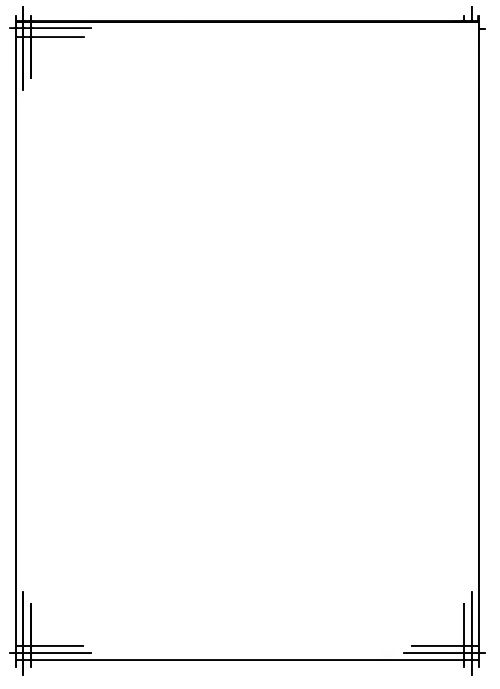
\includegraphics[width=\paperwidth, height=\paperheight]{section/pic/bia.jpg}
	}
}

% Thêm câu lệnh tạo Item
%\newcommand{\itemmini}[1]{%
%	\noindent \includegraphics[h]{imagefile} #1
%}

% Thêm func nhận xét
\newcommand{\comment}[1]{
	\noindent \textbf{Comment:} #1
}

% Thêm func trả lời câu hỏi
\newcounter{questionnumber}
\newenvironment{question}{
	\stepcounter{questionnumber}
	\textbf{Question Experiment \thequestionnumber}
	\begin{enumerate}[leftmargin=*, label = Question \arabic*. ]
	}{
	\end{enumerate}
}

% Môi trường cho câu trả lời
\newenvironment{answer}{
	\vspace{5pt}
	\textbf{Answer:} 
	\begin{itshape}
	}{
	\end{itshape}
	\vspace{10pt}
}

% discussion 
\newenvironment{discussion}{
	\textbf{Discussion}
	\begin{itemize}[label = -]
	}{\end{itemize}}


\begin{document}
	\BgThispage
\thispagestyle{empty}
\begin{center}
	\Large\textbf{ĐẠI HỌC QUỐC GIA THÀNH PHỐ HỒ CHÍ MINH \\ TRƯỜNG ĐẠI HỌC BÁCH KHOA\\--oo0oo--}
\end{center}
\vspace{0.5cm}
\begin{center}
	
\includegraphics[width=0.3\linewidth]{sections/pic/01_logobachkhoatoi.png}
\end{center}
\vspace{0.4cm}
\begin{center}
	\LARGE\textbf{Digital IC Design Laboratory}
	\vspace{0.1cm}
	
	\Large{LAB 1 - MOS TRANSISTOR CHARACTERIZATION}
\end{center}
\vspace{1cm}

\LARGE

\hspace{2cm}\begin{tabular}{p{0.4\linewidth} p{0.5\linewidth}}
	Giảng viên hướng dẫn: & TS. Trần Hoàng Linh \\
						  & Nguyễn Phan Thiên Phúc \\
%						  & Bùi Lê Quốc Doanh \\
%						  & Phan Tấn Khải \\
\end{tabular}

\vspace{0.5cm}
\begin{center}
	Danh sách thành viên nhóm (47)
	
	\begin{tabular}{|c|p{0.4\linewidth}|p{0.2\linewidth}| c |}
		\hline
		STT & Họ và tên & MSSV & Lớp\\
		\hline
		1 & Hà Phước Việt Quốc & 2212832 & L02\\
		\hline
		2 & Nguyễn Tuệ & 2213812 & L02\\
		\hline
		3 & Nguyễn Đại Đồng & 2210780 & L01\\
		\hline
	\end{tabular}
\end{center}

\vspace{1cm}
\begin{center}
	\fontsize{8pt}{5pt}\selectfont\textbf{Tp.HCM, \dots/\dots/20\dots}
\end{center}

\newpage
\thispagestyle{empty}
\fontsize{13}{14}\selectfont
\tableofcontents
\listoffigures
	\section{Experiment 1 - Implement CMOS-based logic gates.}

\subsection{NOT gate}

\subsubsection{Schematic}

\begin{table}[H]
	\centering
	\begin{tabular}{|c|c|}
		\hline
		INPUT & OUTPUT \\
		\hline
		A & B \\
		\hline
		0 & 1 \\
		\hline
		1 & 0\\
		\hline
	\end{tabular}
	\caption{The truth table of an inverter.}
	\label{t_the truth table of inverter}
\end{table}

The schematic of a CMOS-Inverter.

\begin{figure}[H]
	\centering
	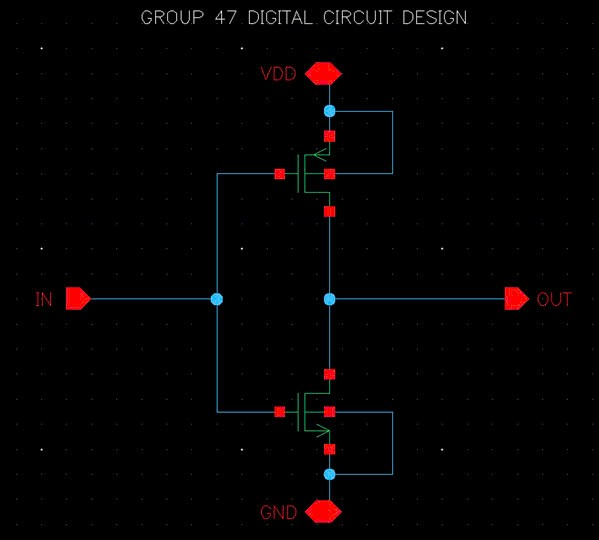
\includegraphics[width=.6\linewidth]{section/EX1/INV/EX1_INV_schematic.png}
	\caption{The schematic of a CMOS-Inverter.}
	\label{f_EX1_INV_schematic}
\end{figure} 

The symbol of a CMOS-Inverter.

\begin{figure}[H]
	\centering
	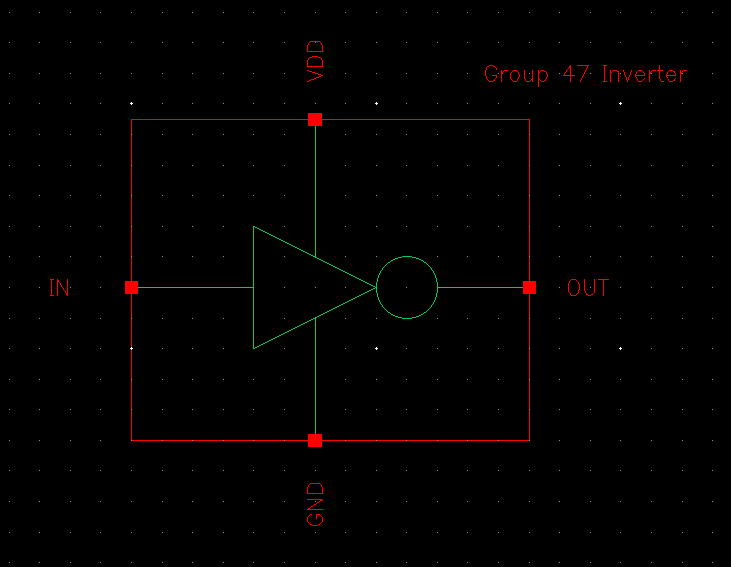
\includegraphics[width=.6\linewidth]{section/EX1/INV/EX1_INV_symbol.png}
	\caption{The symbol of CMOS-Inverter.}
	\label{f_EX1_INV_symbol}
\end{figure}

\subsubsection{DC Analysis simulation}

Use \textbf{ADE-L} to simulate the DC response of an \textit{INV gate}. Apply an input signal as a ramp voltage ranging form 0V to 1V or perform a voltage sweep from 0V to 1V. Observe the corresponding output response. The circuit parameters are configured as follows:

\begin{table}[H]
	\centering
	\begin{tabular}{|c|c|}
		\hline
		Parameters & Value \\
		\hline
		$V_{dd}$ & $1V$ \\
		\hline
		$C_{load}$ & $1fF$\\
		\hline
		$V_{in}$ & $[0, 1] V$\\
		\hline
	\end{tabular}
	\caption{Parameters in DC analysis.}
\end{table}

\begin{figure}[H]
	\centering
	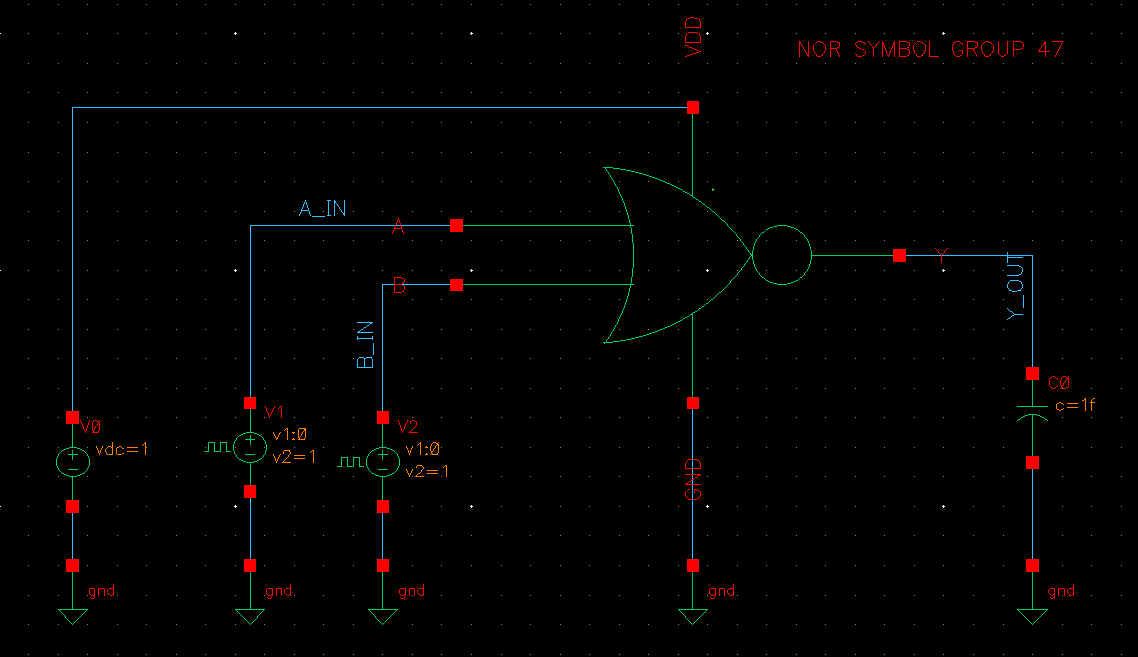
\includegraphics[width=.6\linewidth]{section/EX1/INV/EX1_INV_DCanalysis_schematic.png}
	\caption{The circuit test CMOS-Inverer.}
\end{figure}

\begin{table}[H]
	\centering
	\begin{tabular}{|c|c|c|c|c|c|c|c|c|c|}
		\hline
		$V_{in}(V)$ & $0.1$ & $0.2$ & $0.3$ & $0.4$ & $0.5$ & $0.6$ & $0.7$ & $0.8$ & $0.9$ \\
		\hline
		$V_{out}(V)$ & $999.49m$ & $994.76m$ & $965.48m$ & $846.41m$ & $160.46m$ & $47.237m$ & $15.296m$ & $2.8678m$ & $308.72$ \\
		\hline
	\end{tabular}
	\caption{The output voltage values at various values of $V_{in}$ with $0.1V$ step.}
\end{table}

\begin{figure}[H]
	\centering
	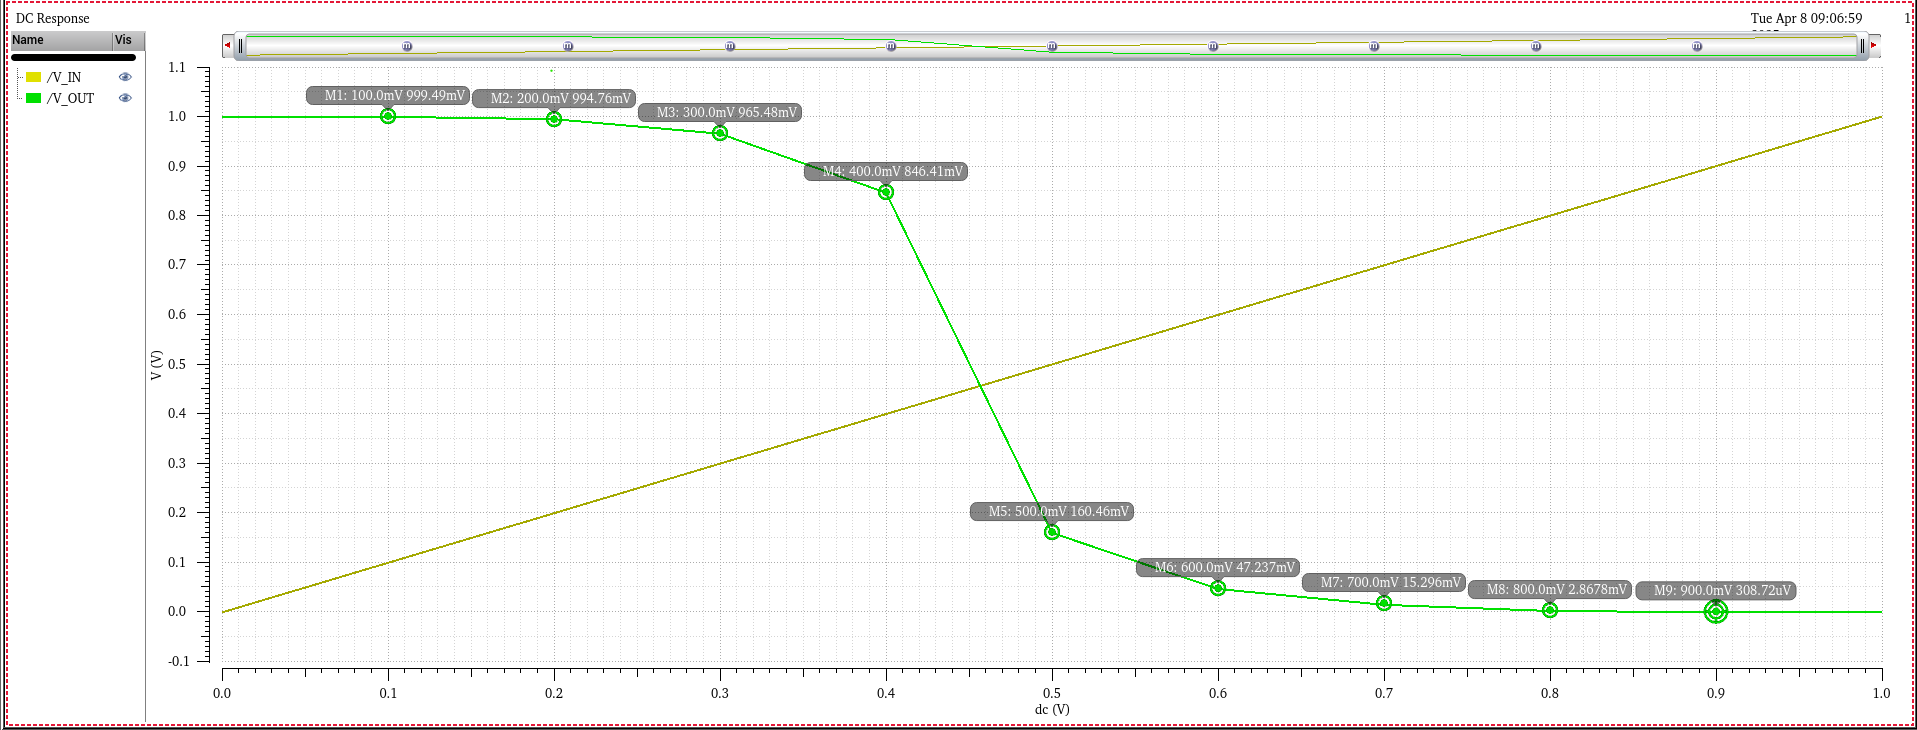
\includegraphics[width=.6\linewidth]{section/EX1/INV/EX1_INV_DCanalysis_vtc.png}
	\caption{Voltage transfer curve (VTC) of CMOS-Inverter.}
	\label{f_EX1_INV_DCanalysis_vtc}
\end{figure}

\subsubsection{Transient simulation}

\begin{figure}[H]
	\centering
	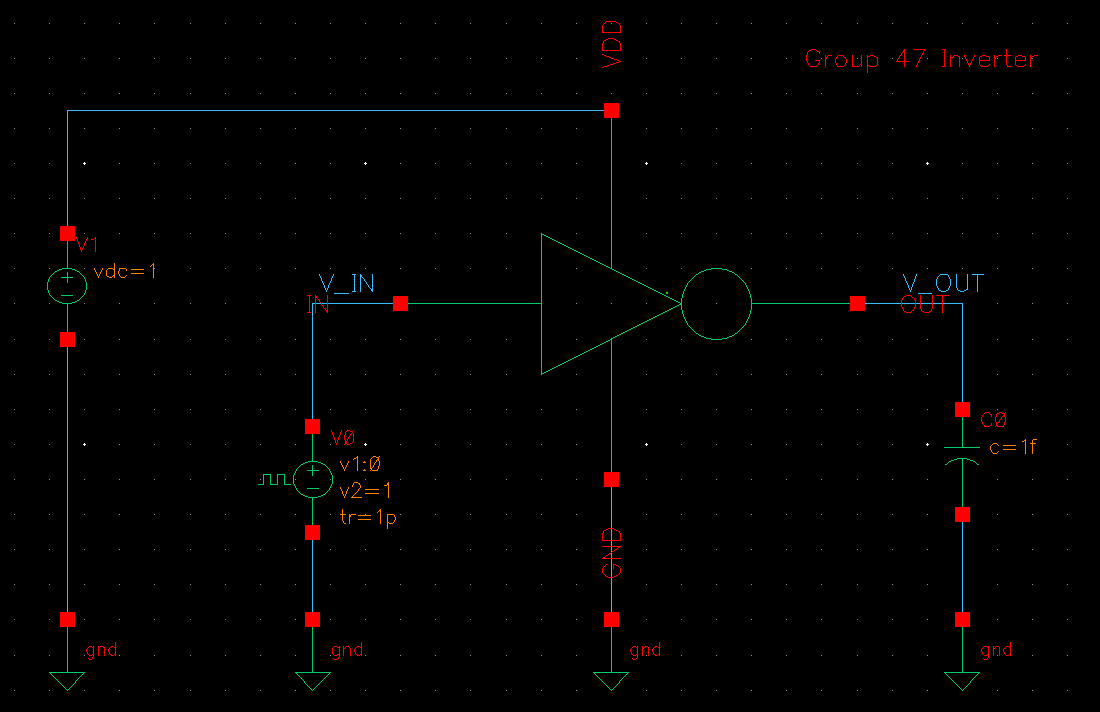
\includegraphics[width=.6\linewidth]{section/EX1/INV/EX1_INV_Trans_schematic.png}
	\caption{The Circuit test CMOS-Inverter.}
\end{figure}

\begin{figure}[H]
	\centering
	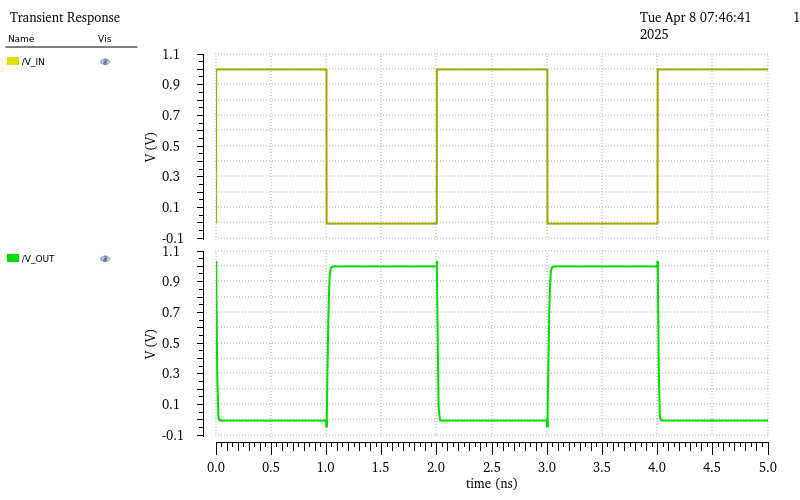
\includegraphics[width=.6\linewidth]{section/EX1/INV/EX1_INV_waveform.png}
	\caption{The waveform CMOS-Inverter.}
	\label{f_EX1_INV_waveform}
\end{figure}

\begin{table}[H]
	\centering
	\begin{tabular}{|p{.5\linewidth}|c|}
		\hline
		Parameters & Result\\
		\hline
		$t_{rise}$ - Rising time ($10\% - 90\%$) & $22.47\times10^{-12}$\\
		\hline
		$t_{fall}$  Falling time ($90\% - 10\%$) & $13.937\times10^{-12}$\\
		\hline
		$t_{pdr}$ - Rising propagation delay ($90\% - 50\%$) & $12.8\times10^{-12}$\\
		\hline
		$t_{pdf}$ - Falling propagation delay ($10\% - 50\%$) & $8.114\times10^{-12}$\\
		\hline
		$t_{p}$ - Average propagation delay ($50\% - 50\%$) & $10.457\times10^{-12}$\\
		\hline
		Dynamic Power & $0$\\
		\hline
		Static Power & $0$\\
		\hline
	\end{tabular}
	\caption{Requirements for measuring INV.}
	\label{f_measuring INV}
\end{table}

\begin{figure}[H]
	\begin{minipage}{0.5\linewidth}
		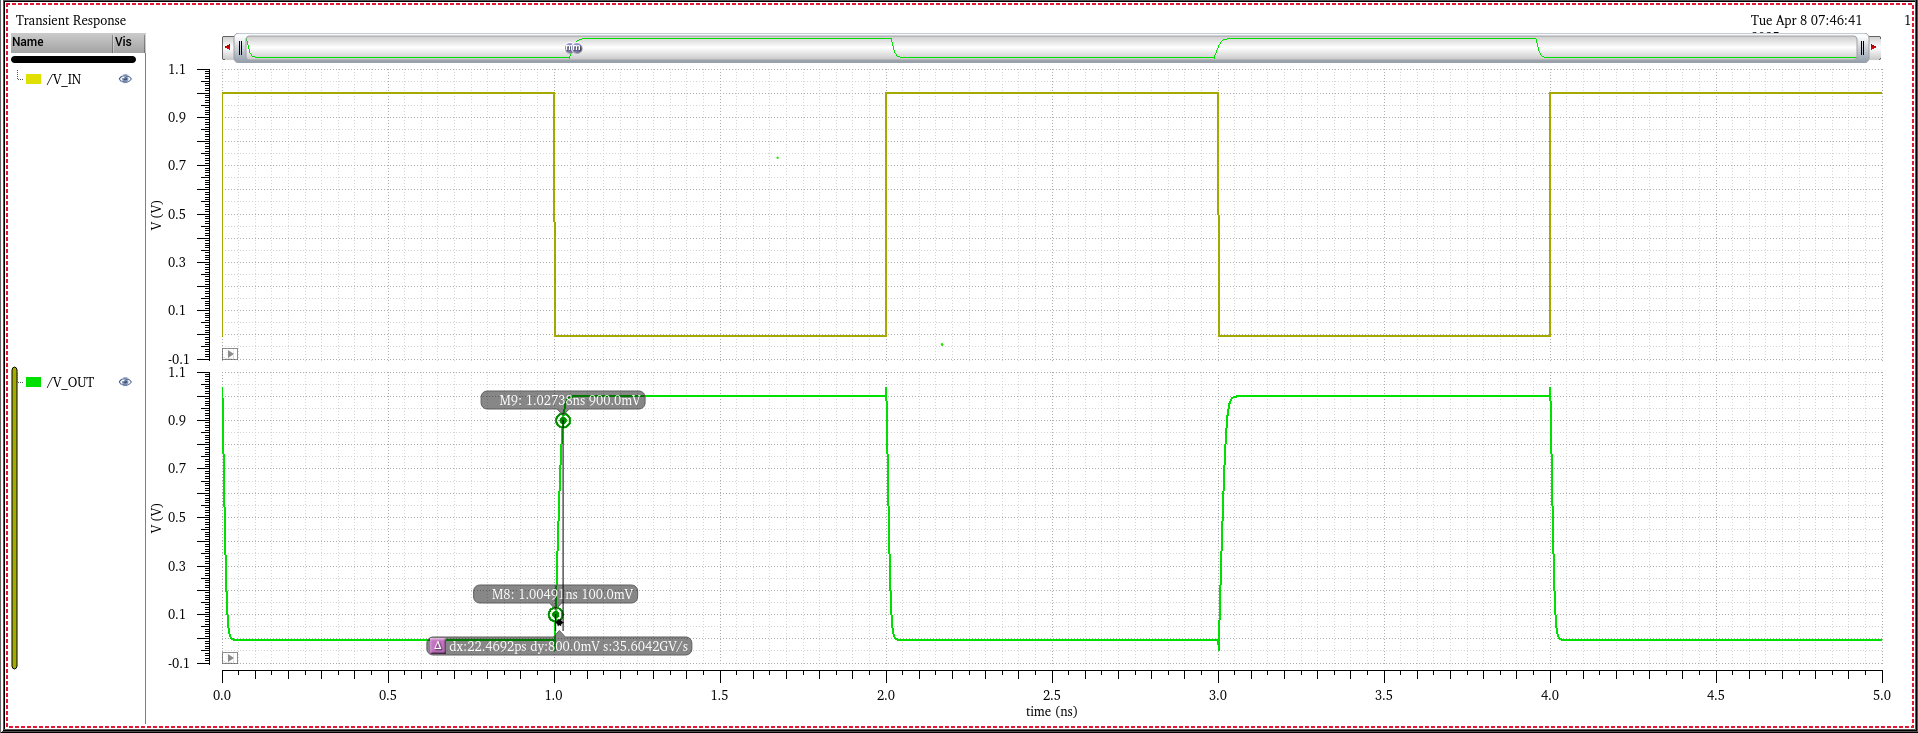
\includegraphics[width=\linewidth]{section/EX1/INV/EX1_INV_Tr_Waveform.png}
	\end{minipage}
	\begin{minipage}{0.5\linewidth}
		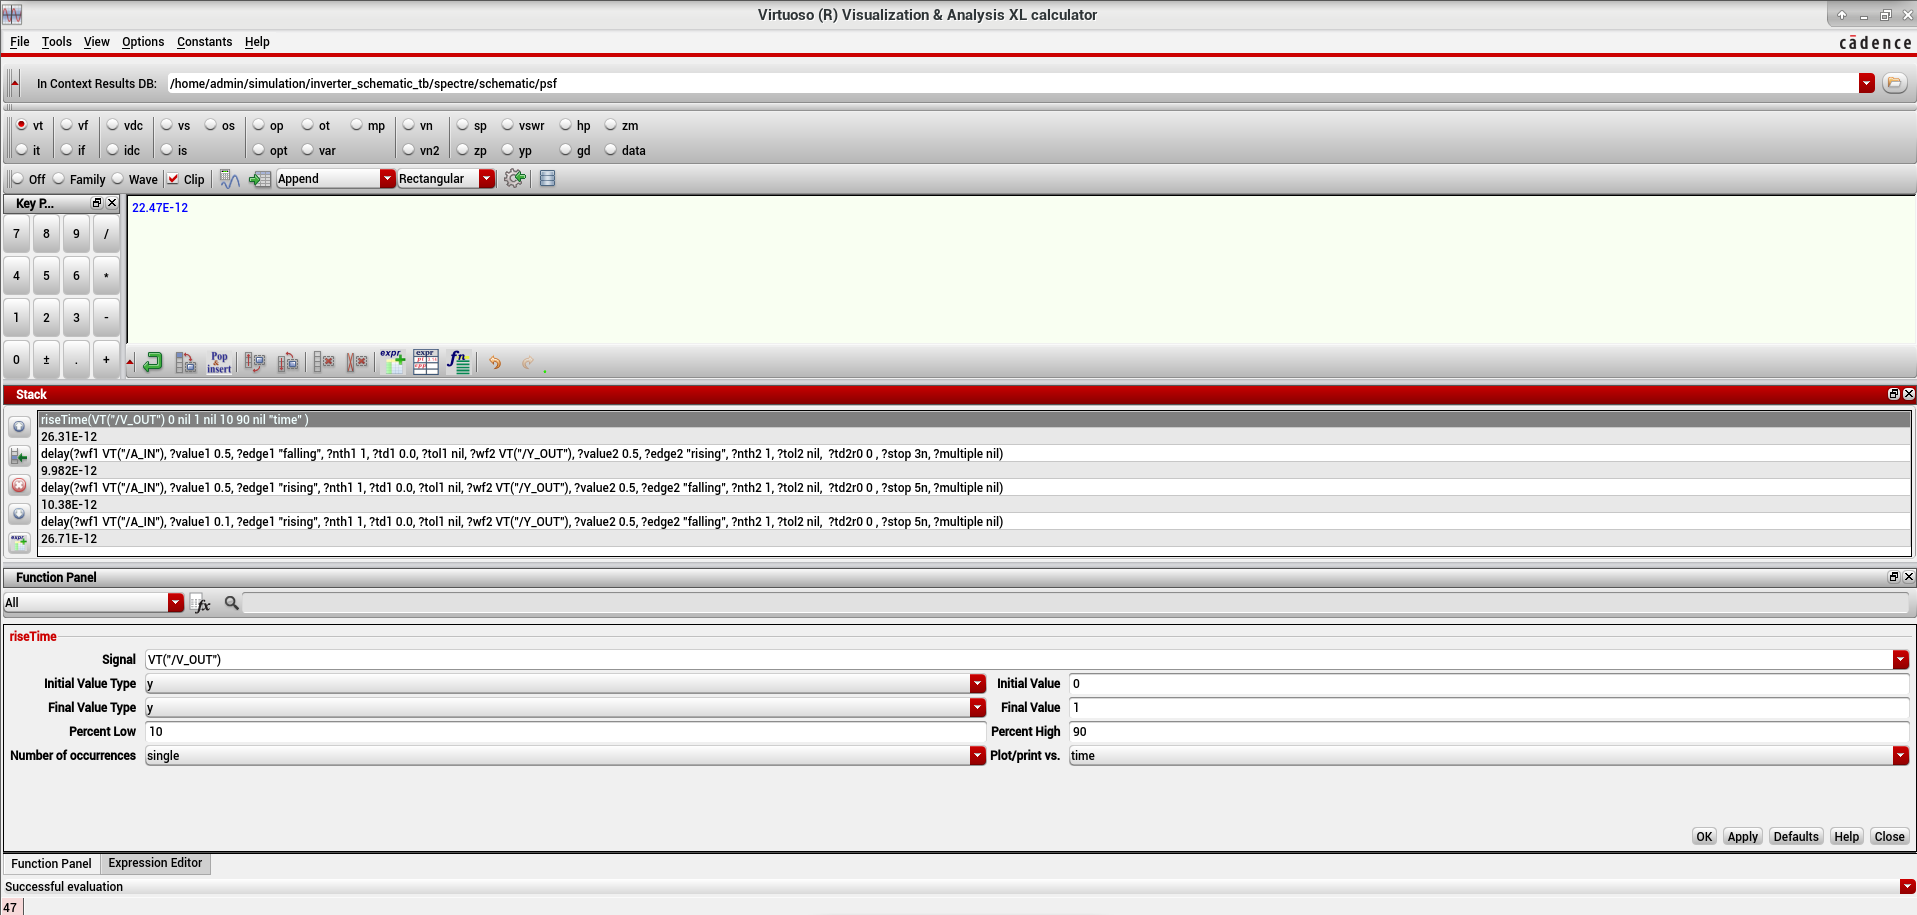
\includegraphics[width=\linewidth]{section/EX1/INV/EX1_INV_Tr_Cal.png}
	\end{minipage}
	\caption{Measurement Time rising INV.}
\end{figure}

\begin{figure}[H]
	\begin{minipage}{0.5\linewidth}
		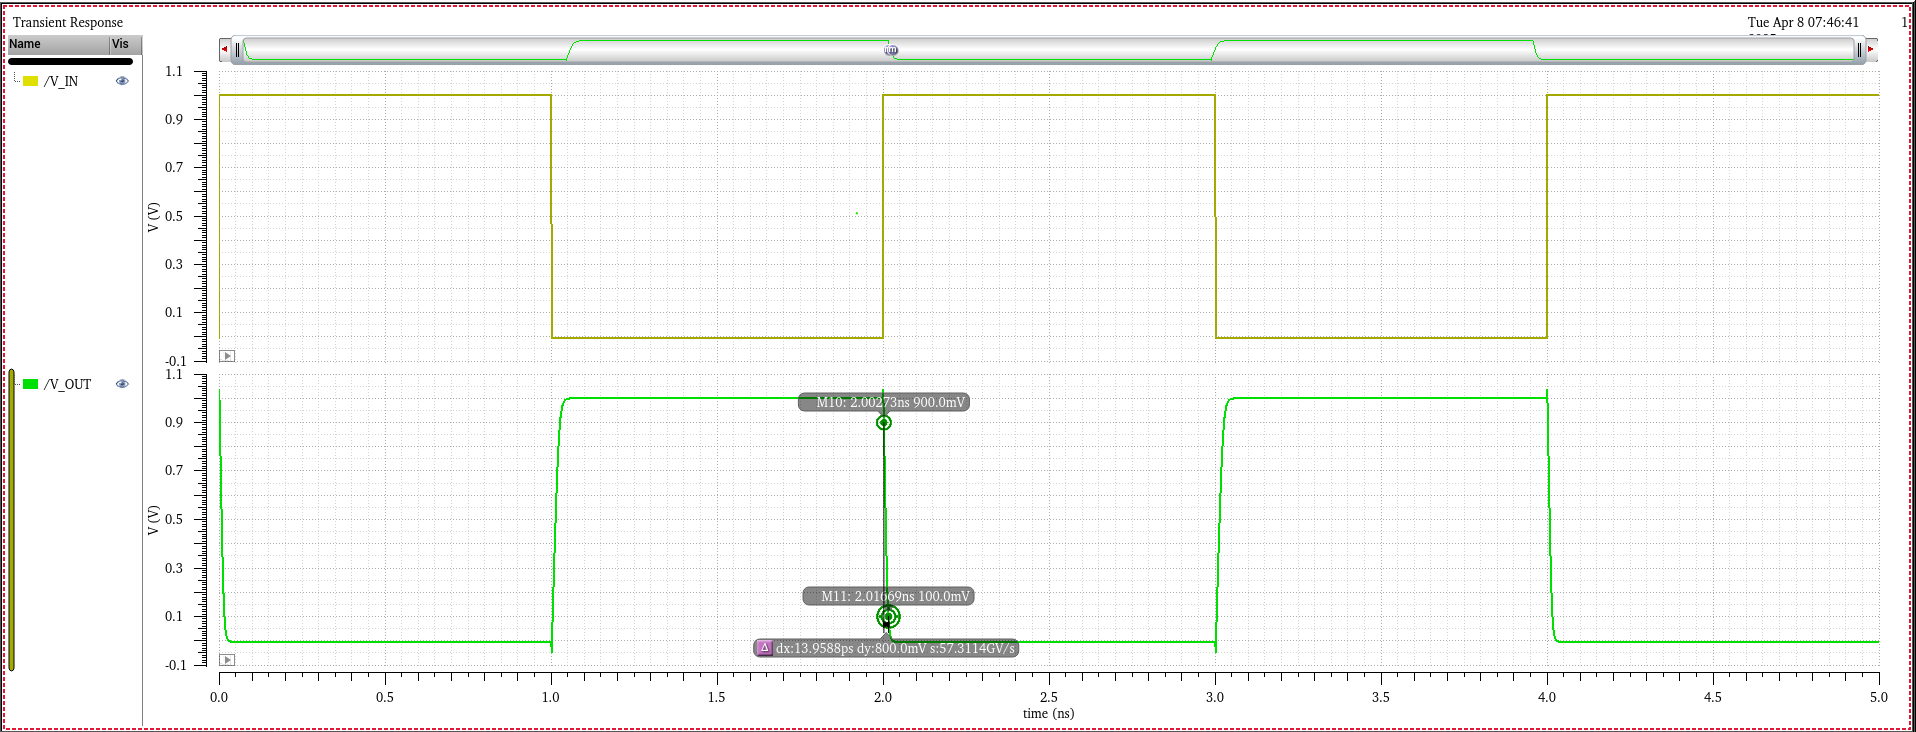
\includegraphics[width=\linewidth]{section/EX1/INV/EX1_INV_Tf_Waveform.png}
	\end{minipage}
	\begin{minipage}{0.5\linewidth}
		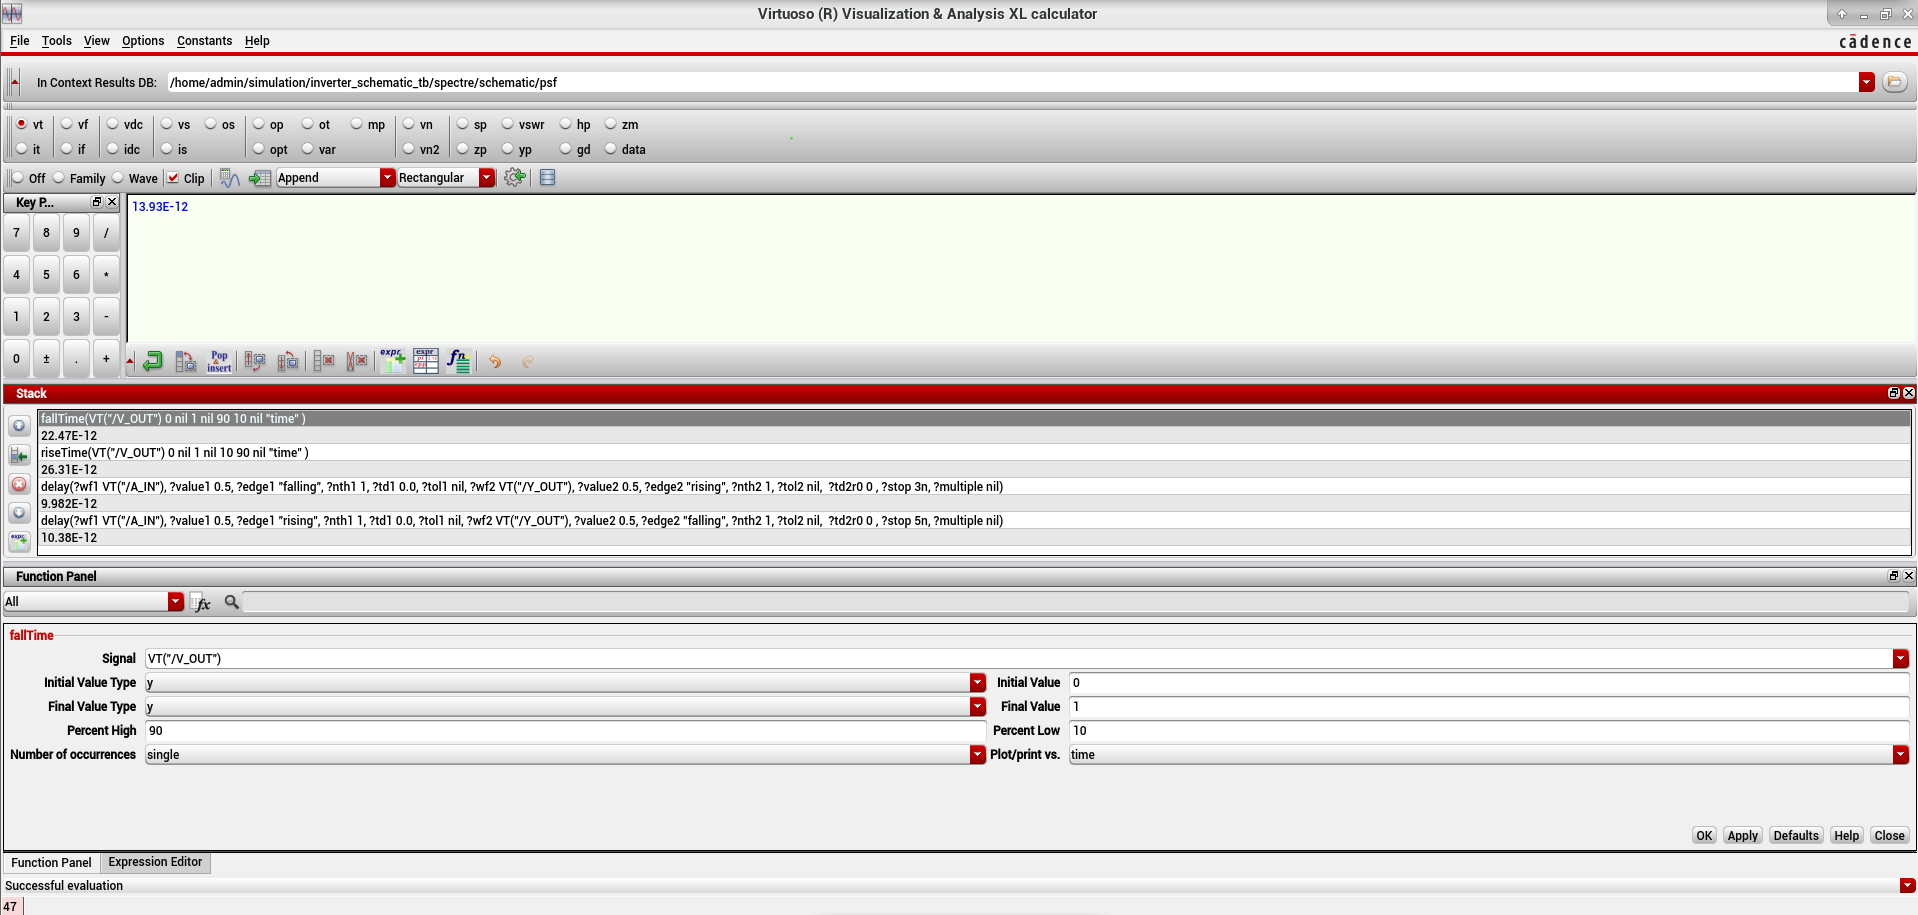
\includegraphics[width=\linewidth]{section/EX1/INV/EX1_INV_Tf_Cal.png}
	\end{minipage}
	\caption{Measurement Time falling INV.}
\end{figure}

\begin{figure}[H]
	\begin{minipage}{0.5\linewidth}
		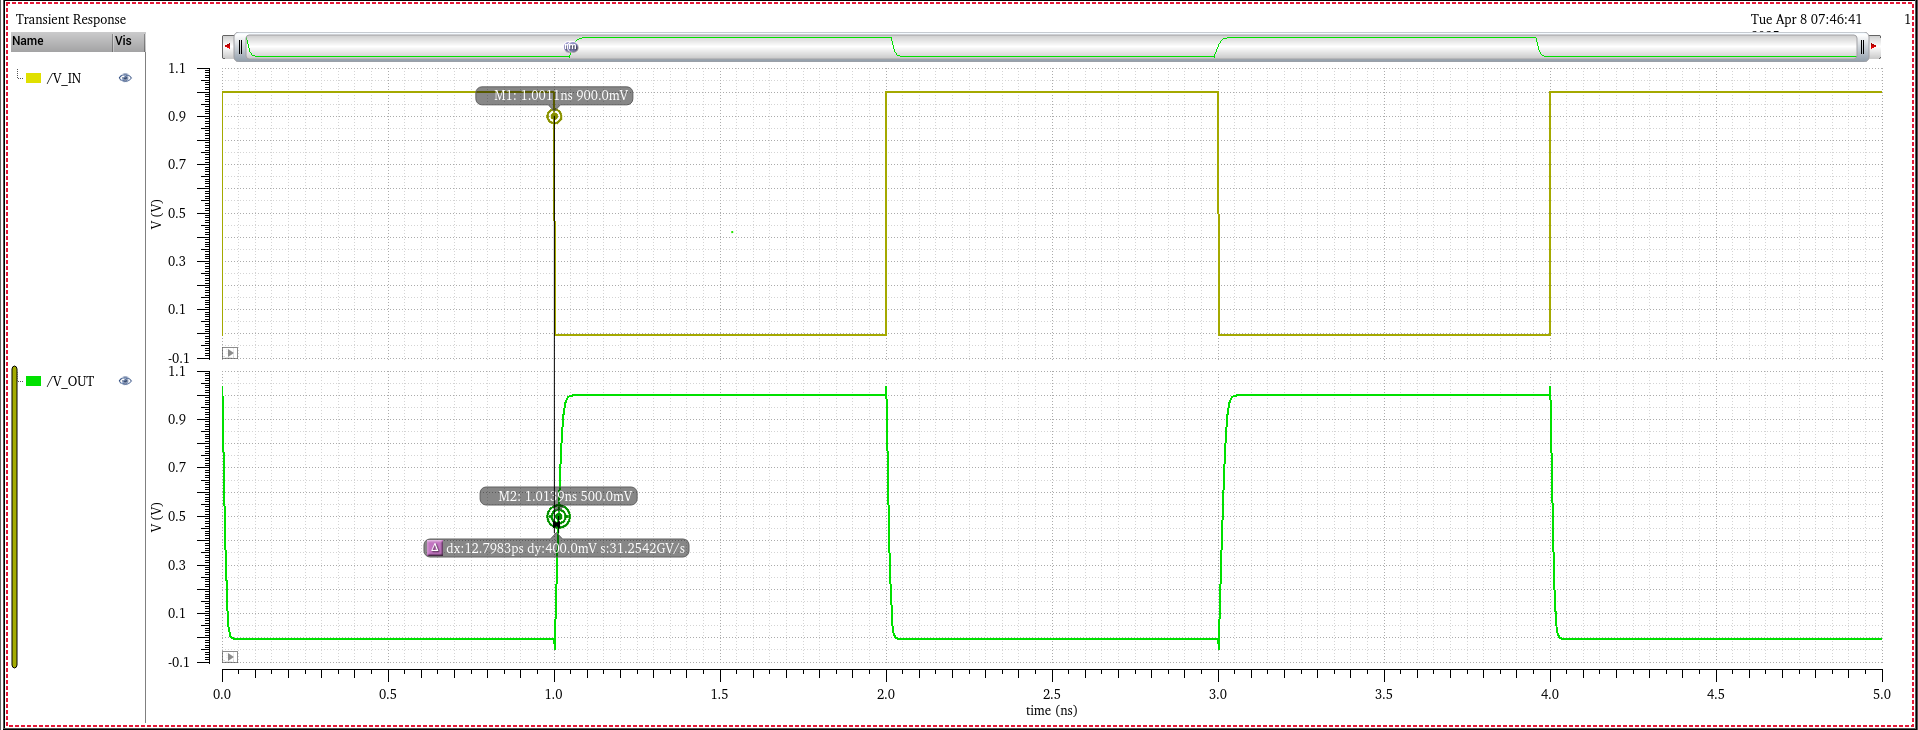
\includegraphics[width=\linewidth]{section/EX1/INV/EX1_INV_Tpdr_Waveform.png}
	\end{minipage}
	\begin{minipage}{0.5\linewidth}
		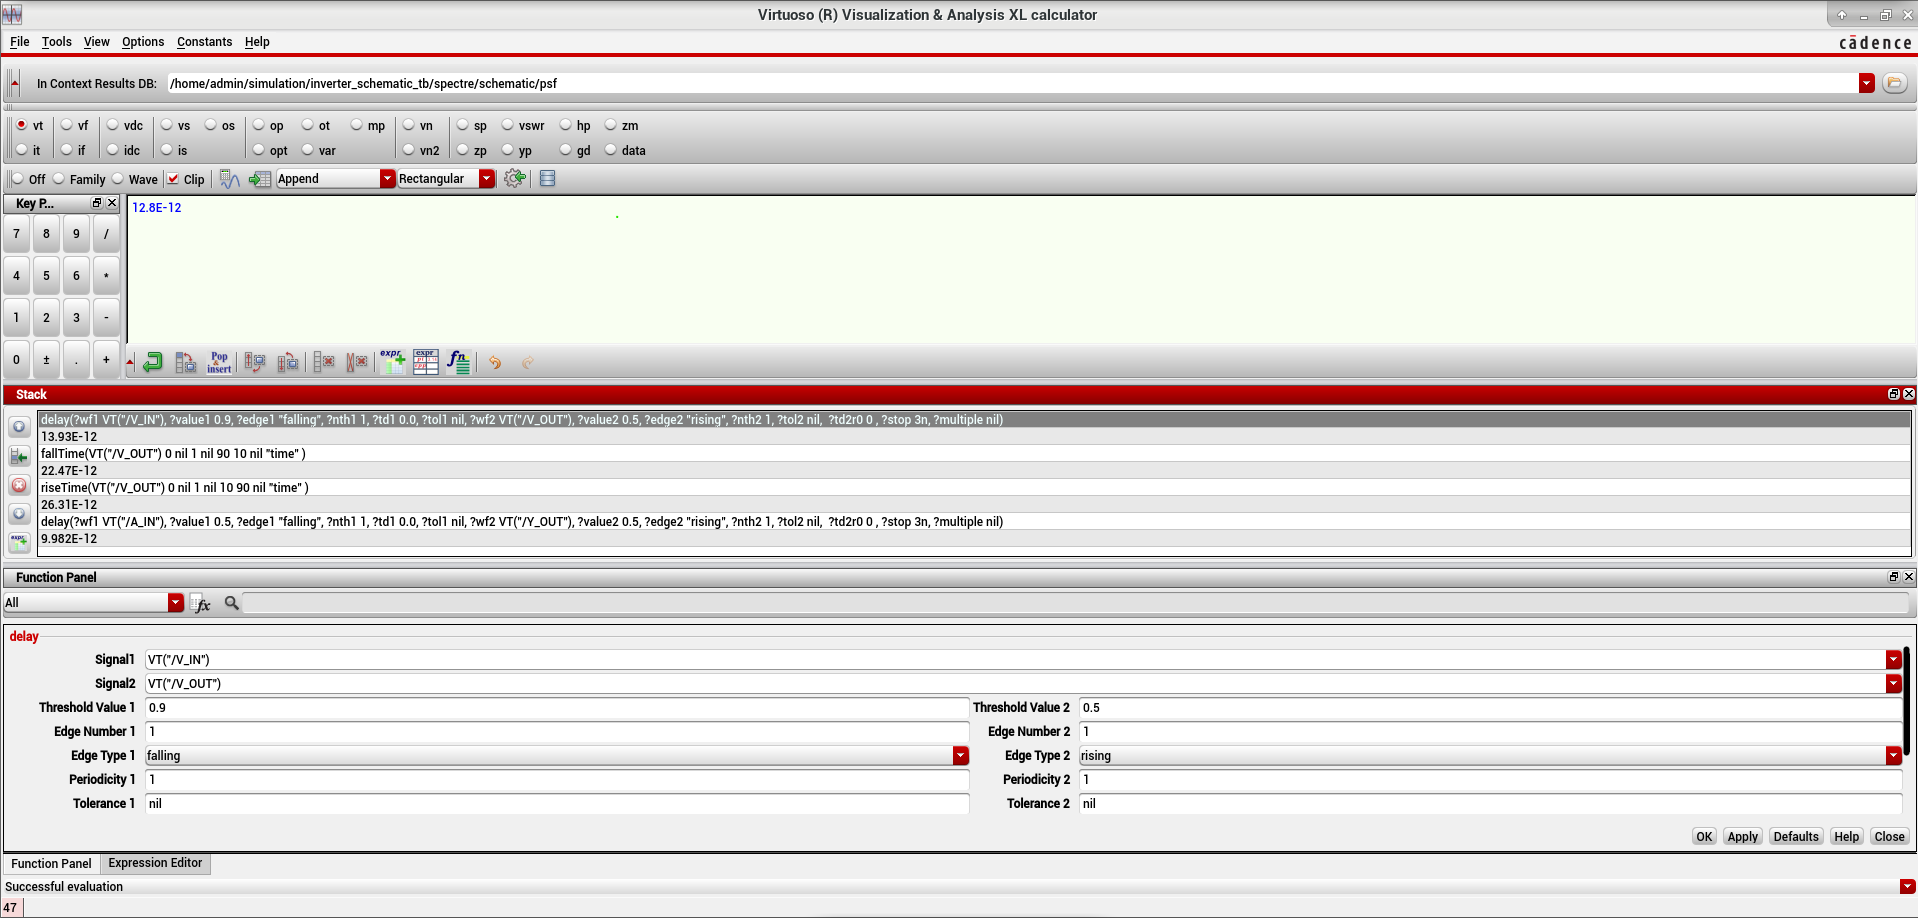
\includegraphics[width=\linewidth]{section/EX1/INV/EX1_INV_Tpdr_Cal.png}
	\end{minipage}
	\caption{Measurement Time rising propagation INV.}
\end{figure}

\begin{figure}[H]
	\begin{minipage}{0.5\linewidth}
		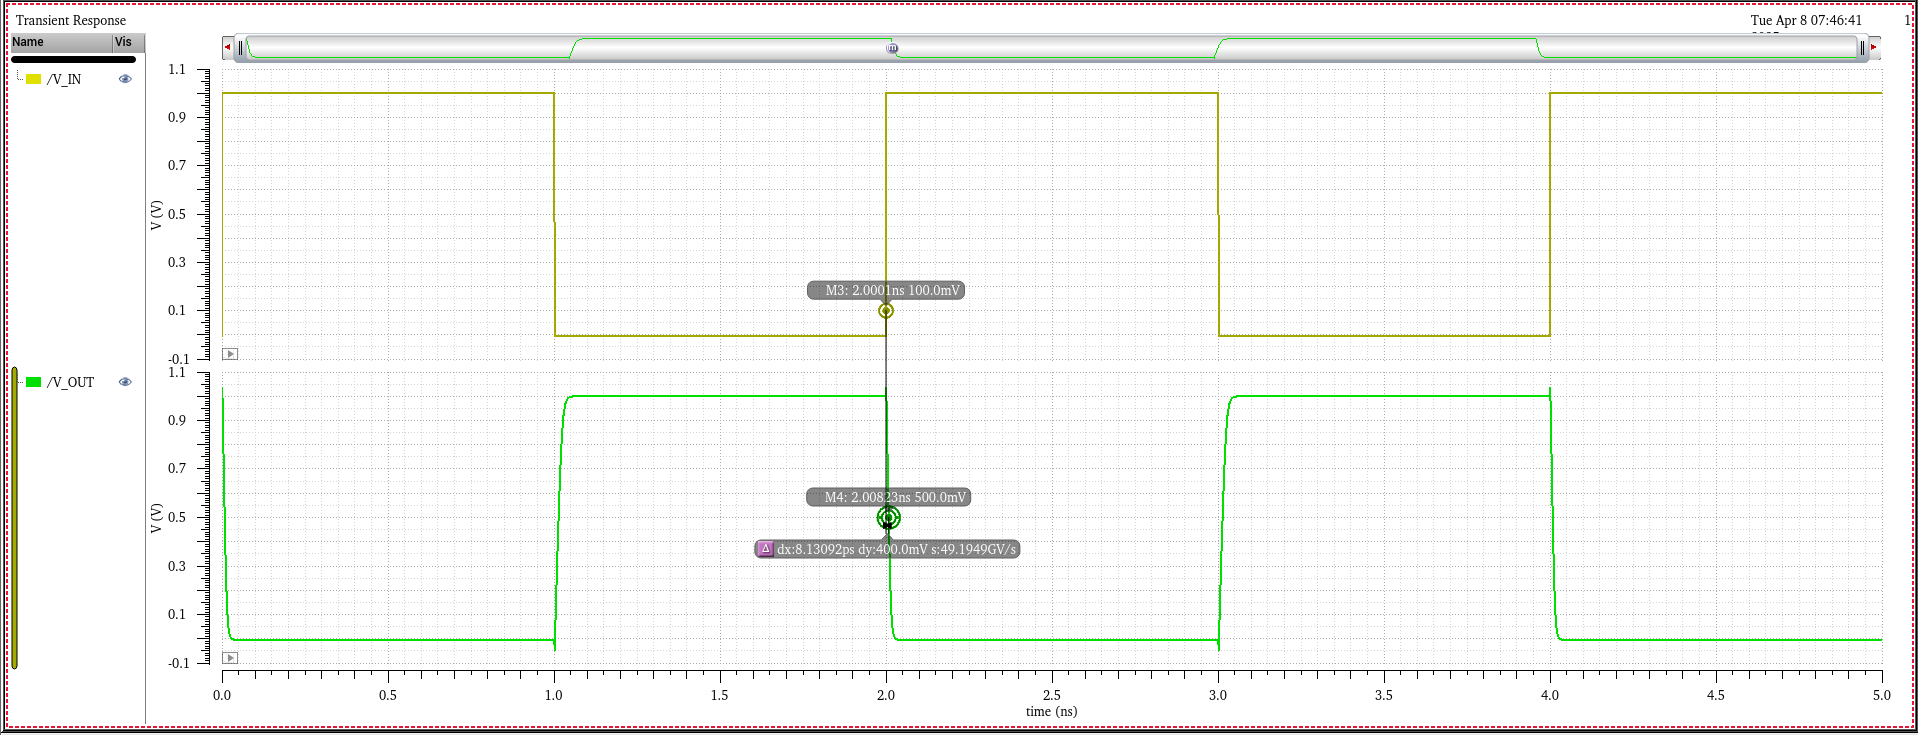
\includegraphics[width=\linewidth]{section/EX1/INV/EX1_INV_Tpdf_Waveform.png}
	\end{minipage}
	\begin{minipage}{0.5\linewidth}
		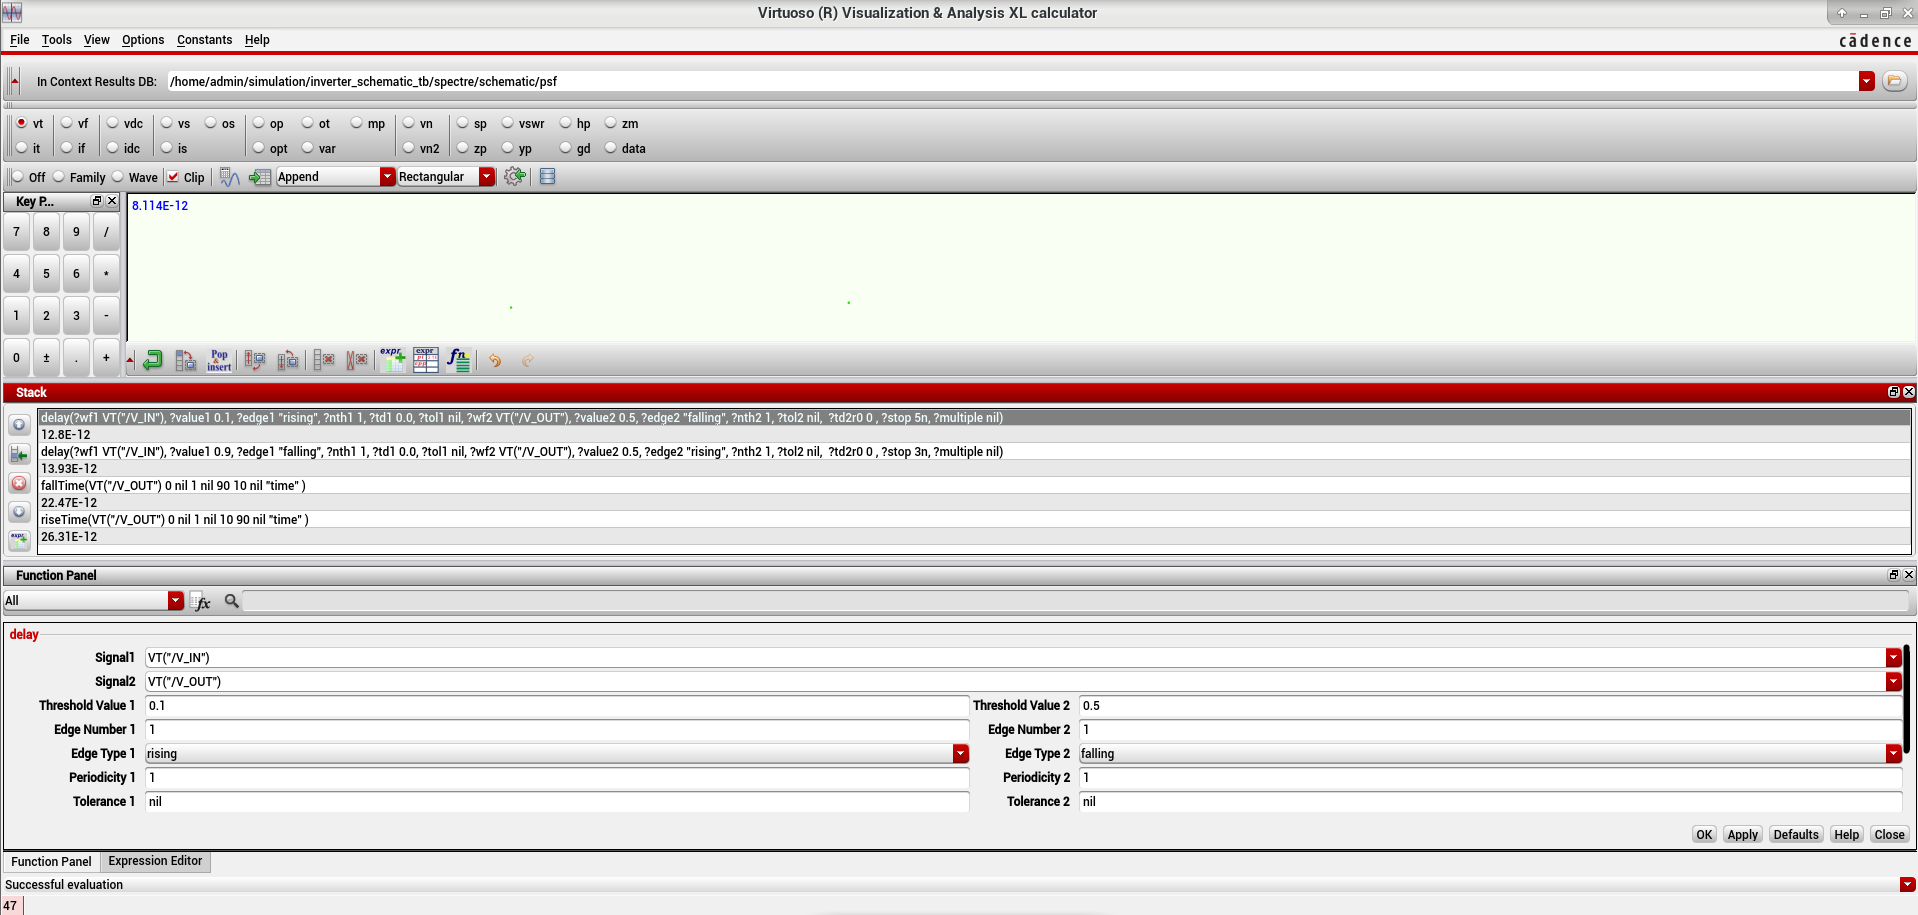
\includegraphics[width=\linewidth]{section/EX1/INV/EX1_INV_Tpdf_Cal.png}
	\end{minipage}
	\caption{Measurement Time falling propagation INV.}
\end{figure}

\subsubsection{Layout of INV}

\begin{figure}[H]
	\centering
	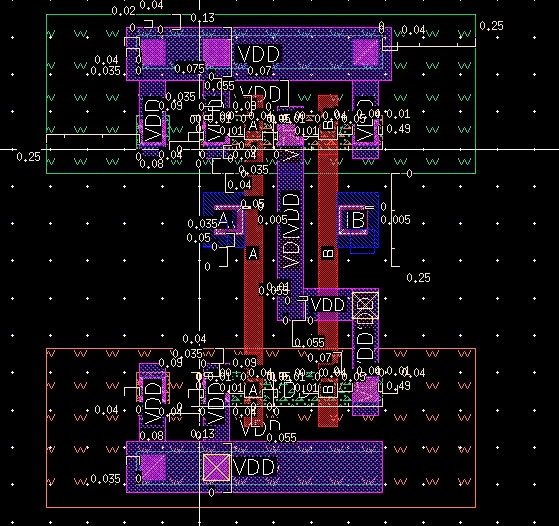
\includegraphics[width=.7\linewidth]{section/EX1/INV/EX1_INV_layout.png}
	\caption{Layout for INV.}
	\label{f_EX1_INV_layout}
\end{figure}

\subsection{NAND2 gate}

\subsubsection{Schematic}

\begin{table}[H]
	\centering
	\begin{tabular}{|c|c|c|}
		\hline
		\multicolumn{2}{|c|}{INPUT} & OUTPUT \\
		\hline
		A & B  & OUT\\
		\hline
		0 & 0 & 1 \\
		\hline
		0 & 1 & 1\\
		\hline
		1 & 0 & 1\\
		\hline
		1 & 1 & 0\\
		\hline
	\end{tabular}
	\caption{The truth table of an NAND2.}
	\label{t_the truth table of NAND2}
\end{table}

The schematic of a NAND2.

\begin{figure}[H]
	\centering
	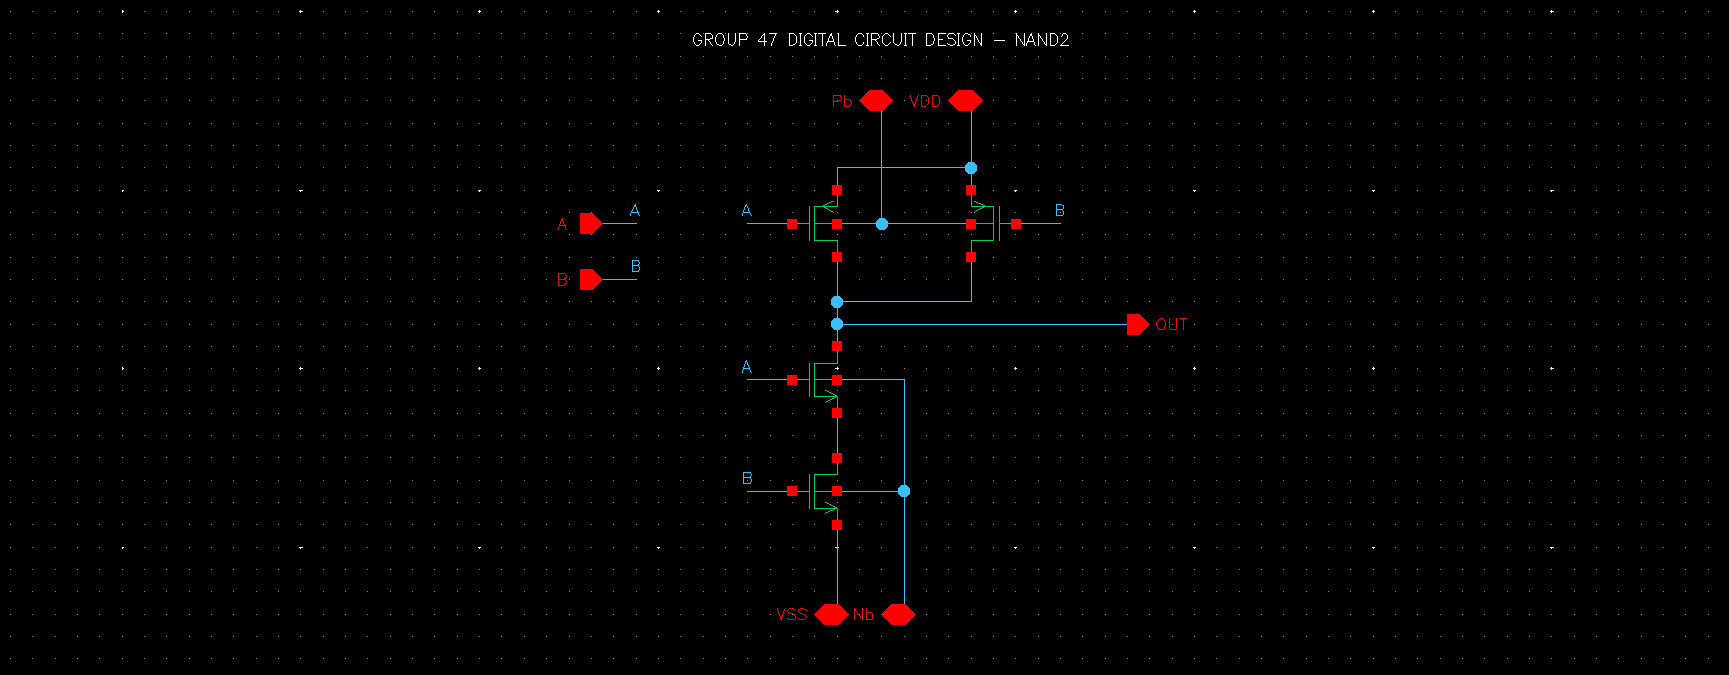
\includegraphics[width=.6\linewidth]{section/EX1/NAND/EX1_NAND2_schematic.png}
	\caption{The schematic of a NAND2.}
	\label{f_EX1_NAND2_schematic}
\end{figure} 

The symbol of a NAND2.

\begin{figure}[H]
	\centering
	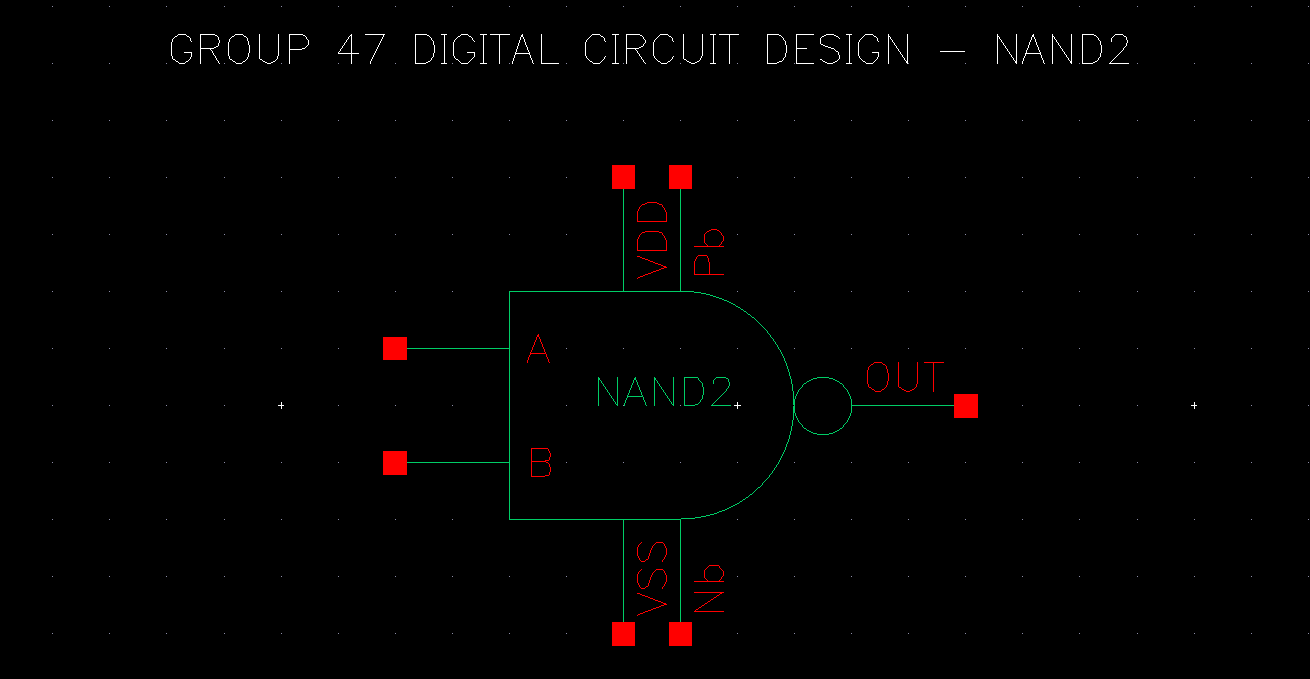
\includegraphics[width=.6\linewidth]{section/EX1/NAND/EX1_NAND2_symbol.png}
	\caption{The symbol of NAND2.}
	\label{f_EX1_NAND2_symbol}
\end{figure}

\subsubsection{DC Analysis simulation}

Use \textbf{ADE-L} to simulate the DC response of an \textit{NAND2 gate}. Apply an input signal as a ramp voltage ranging form 0V to 1V or perform a voltage sweep from 0V to 1V. Observe the corresponding output response. The circuit parameters are configured as follows:

\begin{table}[H]
	\centering
	\begin{tabular}{|c|c|}
		\hline
		Parameters & Value \\
		\hline
		$V_{dd}$ & $1V$ \\
		\hline
		$C_{load}$ & $1fF$\\
		\hline
		$V_{in}$ & $[0, 1] V$\\
		\hline
	\end{tabular}
	\caption{Parameters in DC analysis.}
\end{table}

\begin{figure}[H]
	\centering
	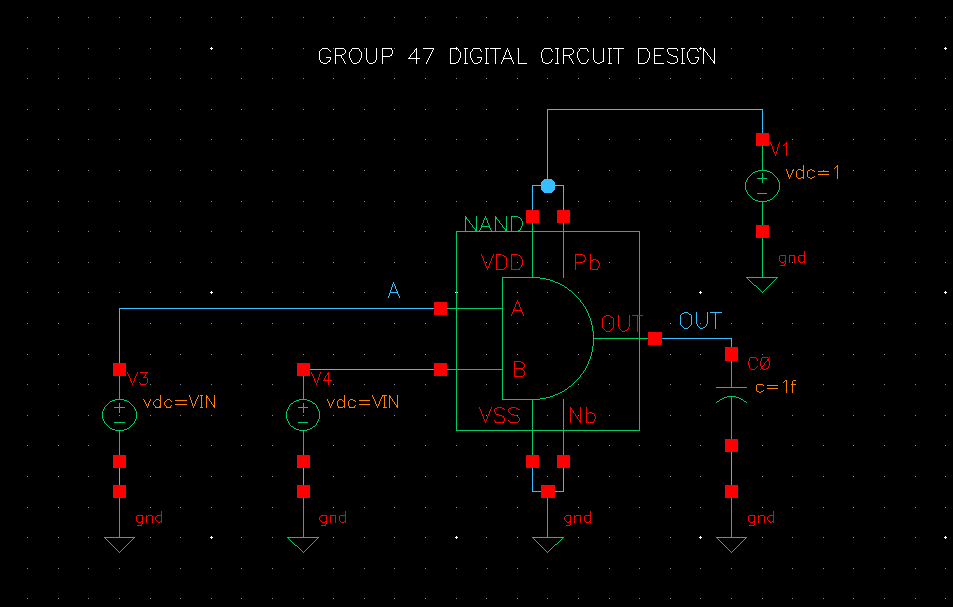
\includegraphics[width=.6\linewidth]{section/EX1/NAND/EX1_NAND2_DCanalysis_schematic.png}
	\caption{The circuit test NAND2.}
\end{figure}

\begin{table}[H]
	\centering
	\begin{tabular}{|c|c|c|c|c|c|c|c|c|c|}
		\hline
		$V_{in}(V)$ & $0.1$ & $0.2$ & $0.3$ & $0.4$ & $0.5$ & $0.6$ & $0.7$ & $0.8$ & $0.9$ \\
		\hline
		$V_{out}(mV)$ & $999.97$ & $999.58$ & $999.02$ & $978.55$ & $919.16$ & $264.14$ & $60.385$ & $11.339$ & $1.1326$ \\
		\hline
	\end{tabular}
	\caption{The output voltage values at various values of $V_{in}$ with $0.1V$ step.}
\end{table}

\begin{figure}[H]
	\centering
	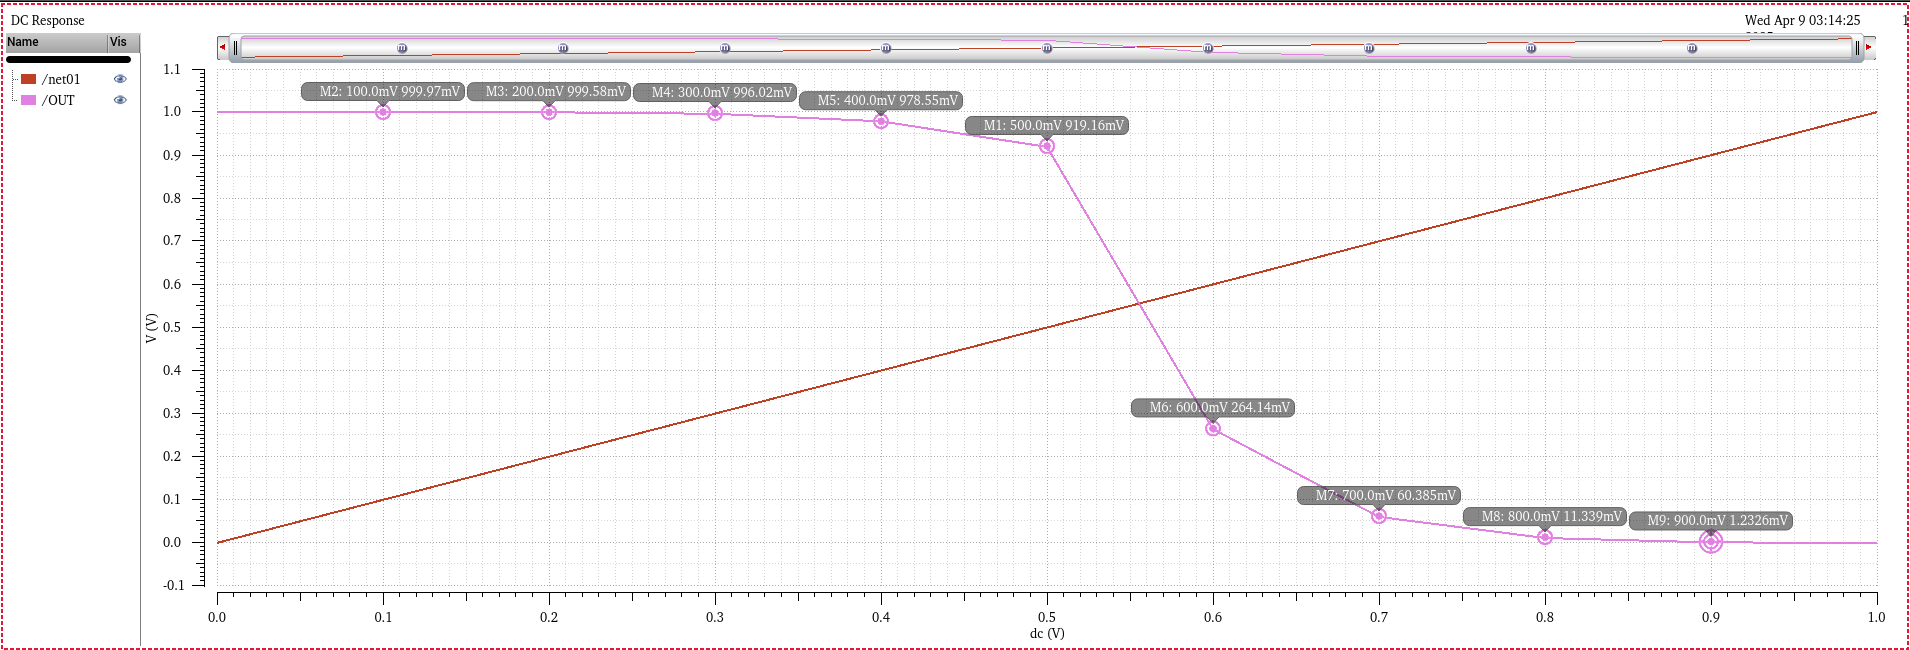
\includegraphics[width=.6\linewidth]{section/EX1/NAND/EX1_NAND2_DCanalysis_vtc.png}
	\caption{Voltage transfer curve (VTC) of NAND2.}
	\label{f_EX1_NAND2_DCanalysis_vtc}
\end{figure}

\subsubsection{Transient simulation}

\begin{figure}[H]
	\centering
	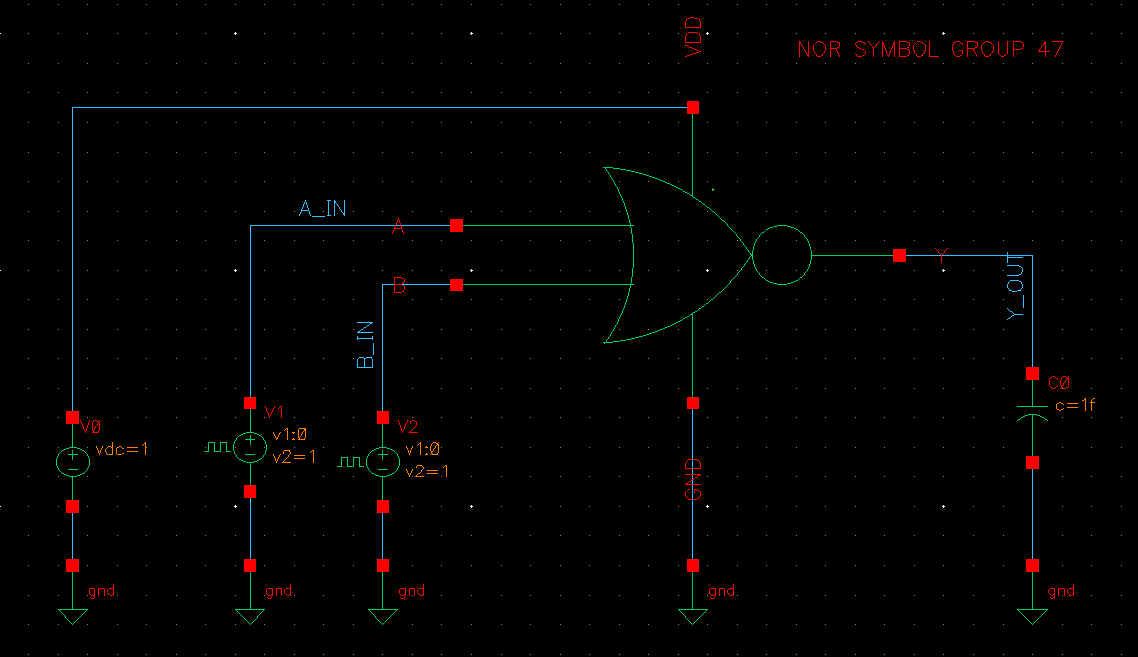
\includegraphics[width=.6\linewidth]{section/EX1/NAND/EX1_NAND2_Trans_schematic.png}
	\caption{The Circuit test NAND2.}
\end{figure}

\begin{figure}[H]
	\centering
	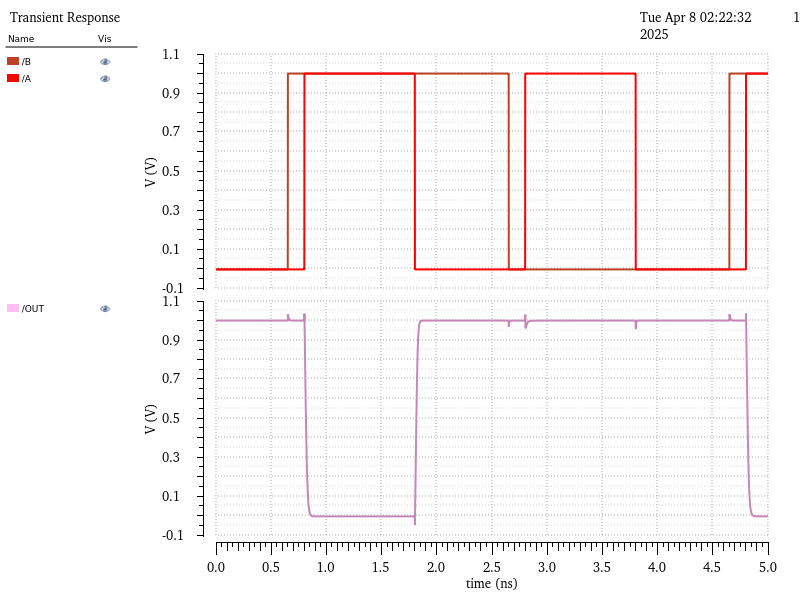
\includegraphics[width=.6\linewidth]{section/EX1/NAND/EX1_NAND2_waveform.png}
	\caption{The waveform NAND2.}
	\label{f_EX1_NAND2_waveform}
\end{figure}

\begin{table}[H]
	\centering
	\begin{tabular}{|p{.5\linewidth}|c|}
		\hline
		Parameters & Result\\
		\hline
		$t_{rise}$ - Rising time ($10\% - 90\%$) & $24.95\times10^{-12}$\\
		\hline
		$t_{fall}$  Falling time ($90\% - 10\%$) & $28.57\times10^{-12}$\\
		\hline
		$t_{pdr}$ - Rising propagation delay ($90\% - 50\%$) & $13.91\times10^{-12}$\\
		\hline
		$t_{pdf}$ - Falling propagation delay ($10\% - 50\%$) & $14.78\times10^{-12}$\\
		\hline
		$t_{p}$ - Average propagation delay ($50\% - 50\%$) & $14.35\times10^{-12}$\\
		\hline
		Power consumption & $0$\\
		\hline
	\end{tabular}
	\caption{Requirements for measuring NAND2.}
	\label{f_measuring NAND2}
\end{table}

\begin{figure}[H]
	\begin{minipage}{0.5\linewidth}
		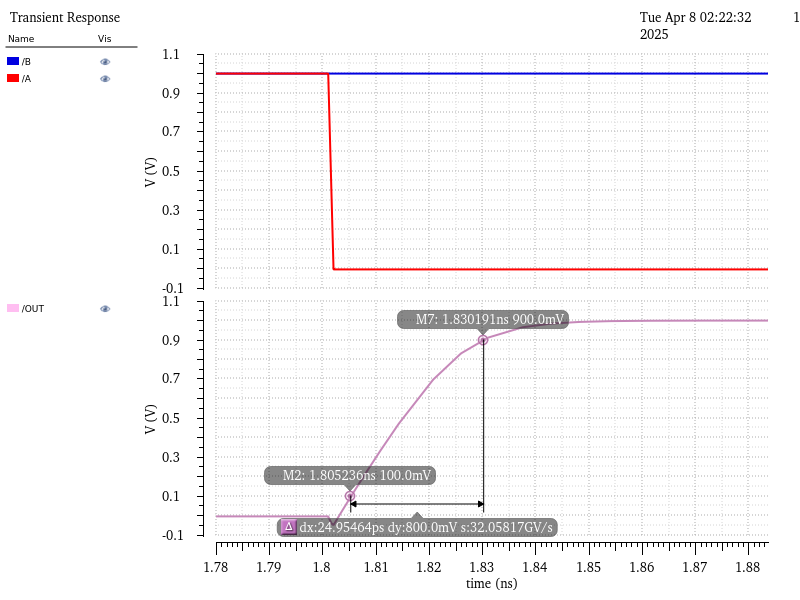
\includegraphics[width=\linewidth]{section/EX1/NAND/EX1_NAND2_Tr_Waveform.png}
	\end{minipage}
	\begin{minipage}{0.5\linewidth}
		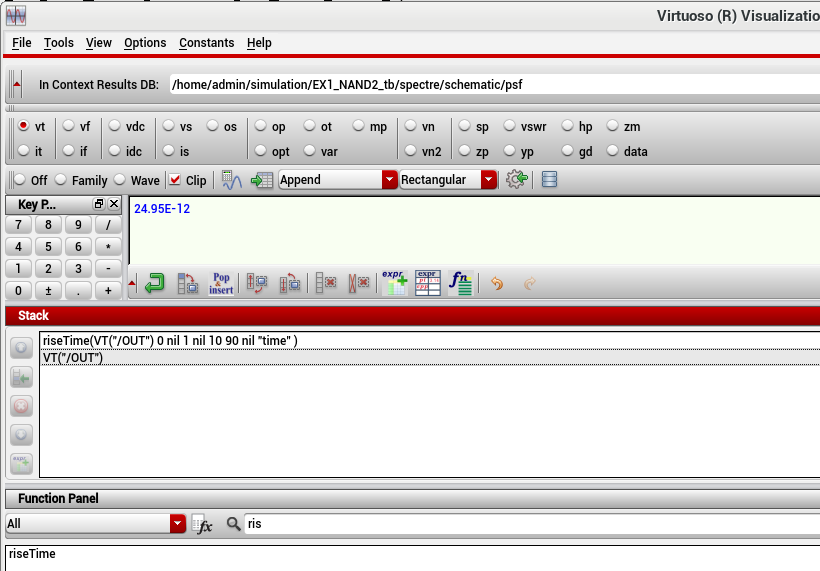
\includegraphics[width=\linewidth]{section/EX1/NAND/EX1_NAND2_Tr_Cal.png}
	\end{minipage}
	\caption{Measurement Time rising NAND2.}
\end{figure}

\begin{figure}[H]
	\begin{minipage}{0.5\linewidth}
		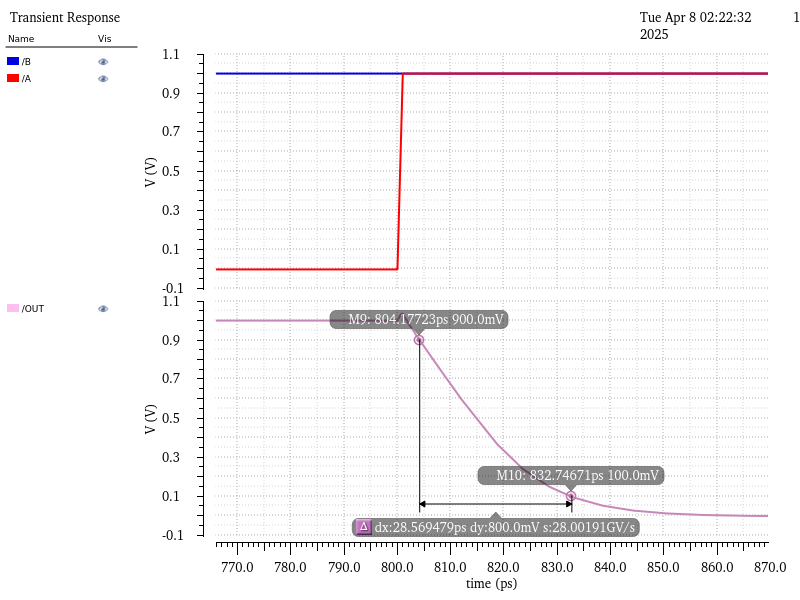
\includegraphics[width=\linewidth]{section/EX1/NAND/EX1_NAND2_Tf_Waveform.png}
	\end{minipage}
	\begin{minipage}{0.5\linewidth}
		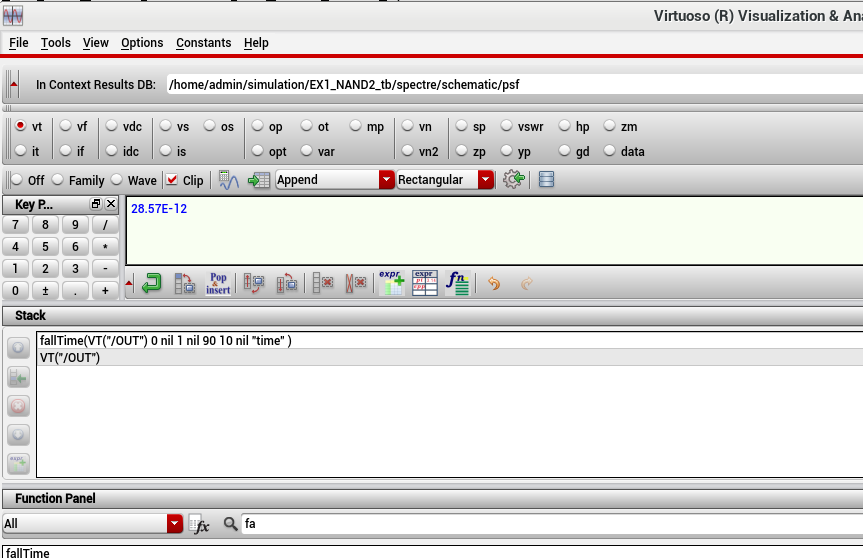
\includegraphics[width=\linewidth]{section/EX1/NAND/EX1_NAND2_Tf_Cal.png}
	\end{minipage}
	\caption{Measurement Time falling NAND2.}
\end{figure}

\begin{figure}[H]
	\begin{minipage}{0.5\linewidth}
		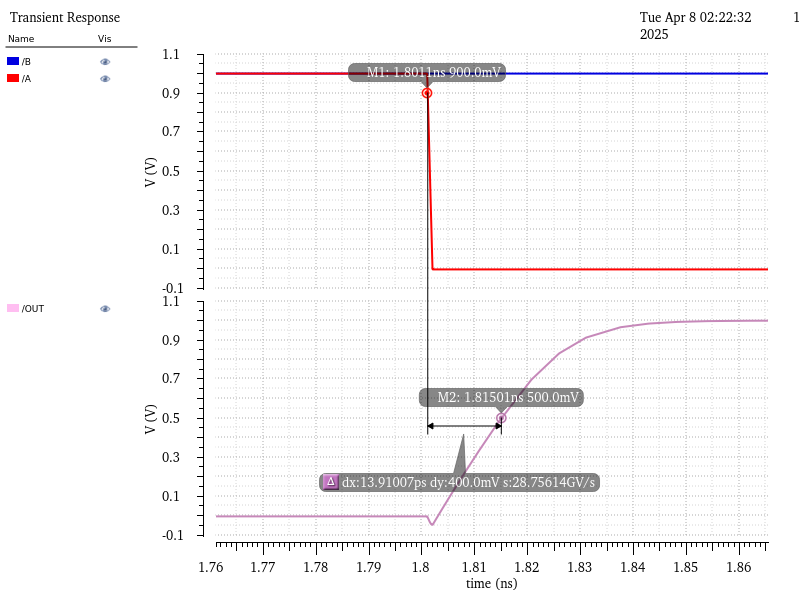
\includegraphics[width=\linewidth]{section/EX1/NAND/EX1_NAND2_Tpdr_Waveform.png}
	\end{minipage}
	\begin{minipage}{0.5\linewidth}
		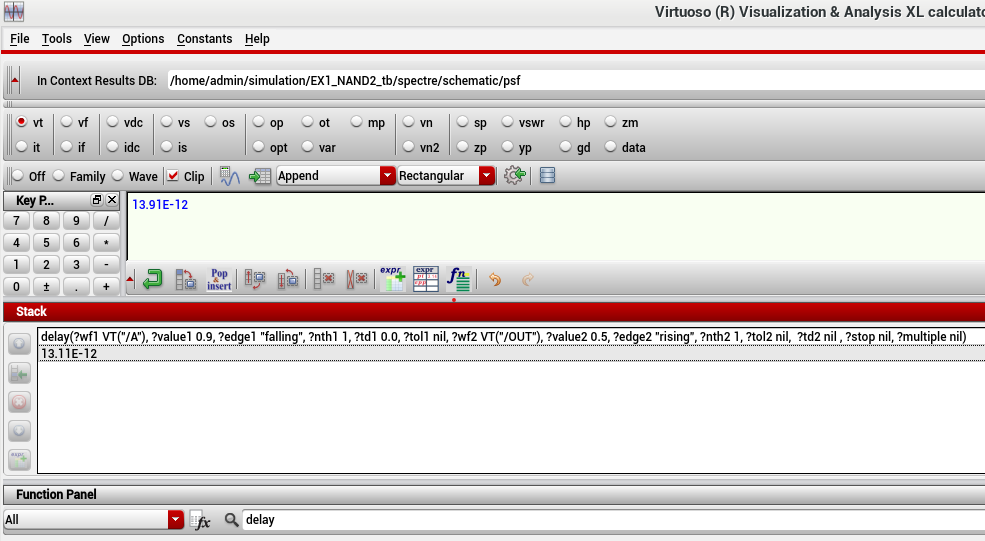
\includegraphics[width=\linewidth]{section/EX1/NAND/EX1_NAND2_Tpdr_Cal.png}
	\end{minipage}
	\caption{Measurement Time rising propagation NAND2.}
\end{figure}

\begin{figure}[H]
	\begin{minipage}{0.5\linewidth}
		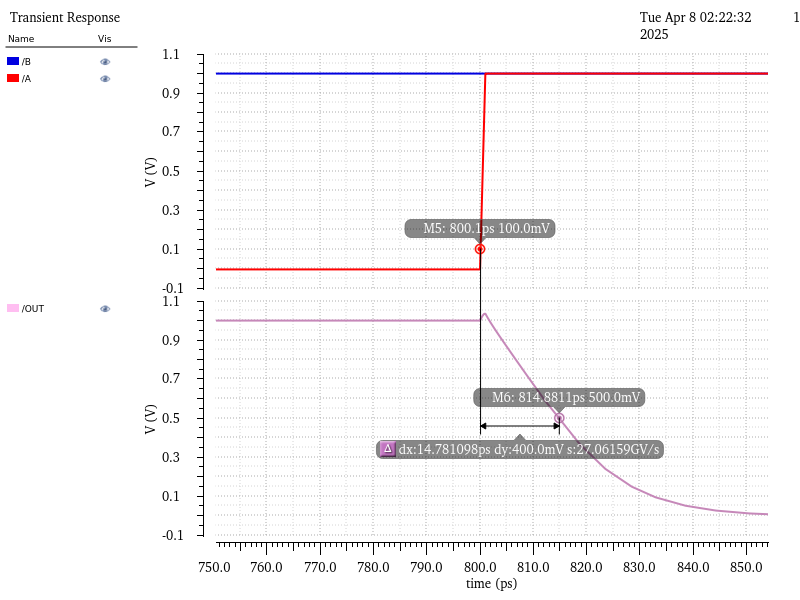
\includegraphics[width=\linewidth]{section/EX1/NAND/EX1_NAND2_Tpdf_Waveform.png}
	\end{minipage}
	\begin{minipage}{0.5\linewidth}
		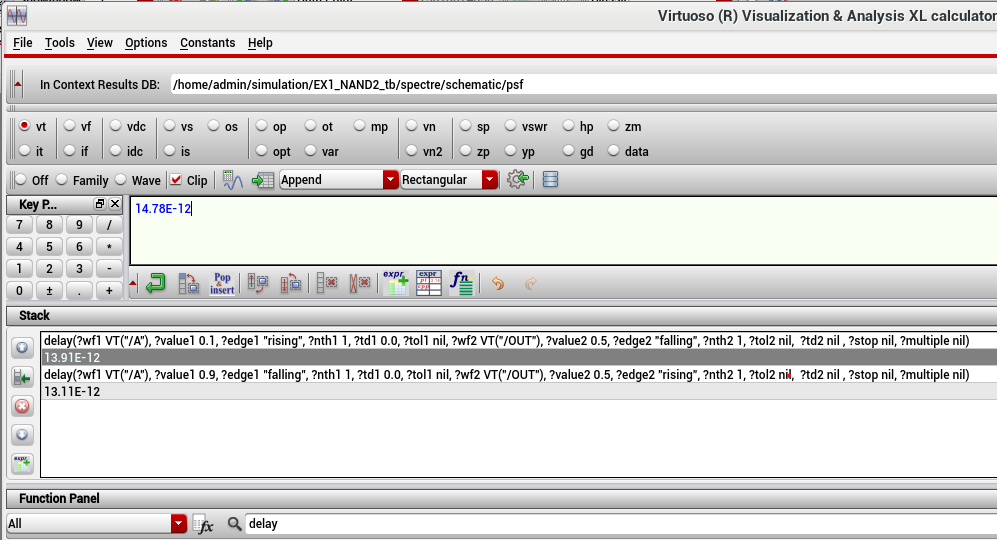
\includegraphics[width=\linewidth]{section/EX1/NAND/EX1_NAND2_Tpdf_Cal.png}
	\end{minipage}
	\caption{Measurement Time falling propagation NAND2.}
\end{figure}

\subsubsection{Layout of NAND2}
\subsection{NOR2 gate}

\subsubsection{Schematic}

\begin{table}[H]
	\centering
	\begin{tabular}{|c|c|c|}
		\hline
		\multicolumn{2}{|c|}{INPUT} & OUTPUT \\
		\hline
		A & B  & OUT\\
		\hline
		0 & 0 & 1 \\
		\hline
		0 & 1 & 0\\
		\hline
		1 & 0 & 0\\
		\hline
		1 & 1 & 0\\
		\hline
	\end{tabular}
	\caption{The truth table of an NOR2.}
	\label{t_the truth table of NOR2}
\end{table}

The schematic of a NOR2.

\begin{figure}[H]
	\centering
	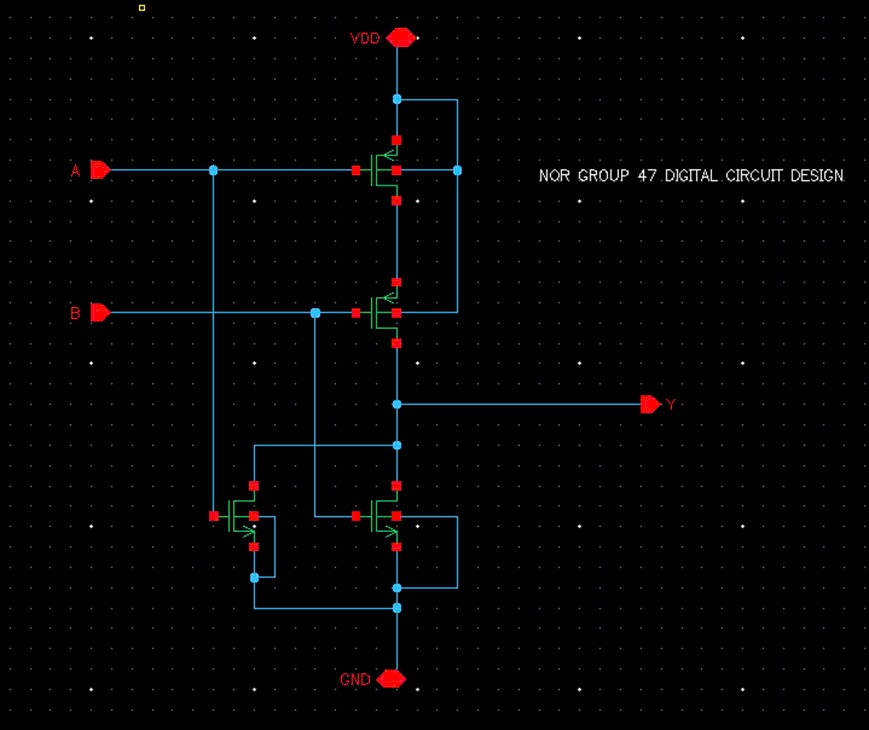
\includegraphics[width=.6\linewidth]{section/EX1/NOR/EX1_NOR2_schematic.png}
	\caption{The schematic of a NOR2.}
	\label{f_EX1_NOR2_schematic}
\end{figure} 

The symbol of a NOR2.

\begin{figure}[H]
	\centering
	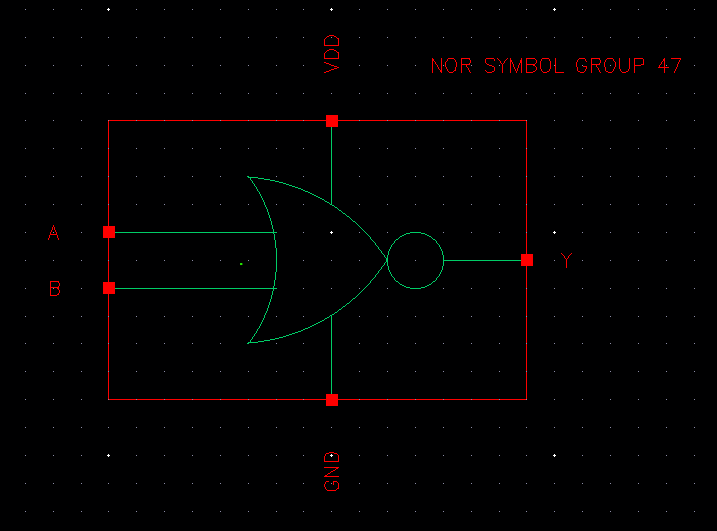
\includegraphics[width=.6\linewidth]{section/EX1/NOR/EX1_NOR2_symbol.png}
	\caption{The symbol of NAND2.}
	\label{f_EX1_NOR2_symbol}
\end{figure}

\subsubsection{DC Analysis simulation}

Use \textbf{ADE-L} to simulate the DC response of an \textit{NOR2 gate}. Apply an input signal as a ramp voltage ranging form 0V to 1V or perform a voltage sweep from 0V to 1V. Observe the corresponding output response. The circuit parameters are configured as follows:

\begin{table}[H]
	\centering
	\begin{tabular}{|c|c|}
		\hline
		Parameters & Value \\
		\hline
		$V_{dd}$ & $1V$ \\
		\hline
		$C_{load}$ & $1fF$\\
		\hline
		$V_{in}$ & $[0, 1] V$\\
		\hline
	\end{tabular}
	\caption{Parameters in DC analysis.}
\end{table}

\begin{figure}[H]
	\centering
	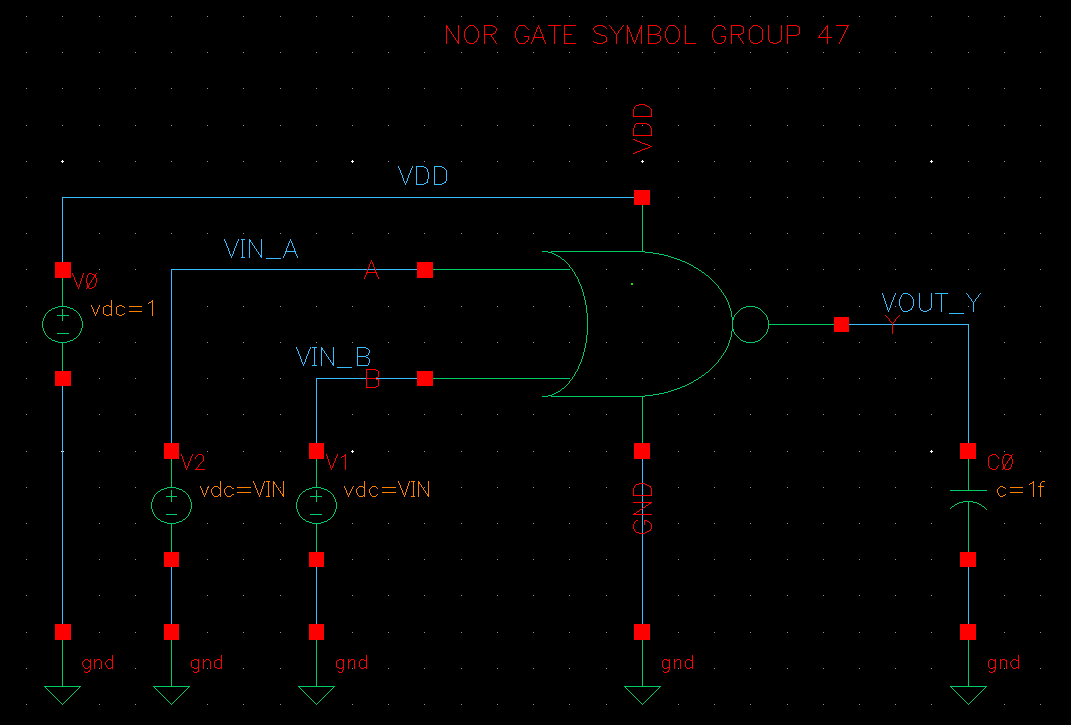
\includegraphics[width=.6\linewidth]{section/EX1/NOR/EX1_NOR2_DCanalysis_schematic.png}
	\caption{The circuit test NOR2.}
\end{figure}

\begin{table}[H]
	\centering
	\begin{tabular}{|c|c|c|c|c|c|c|c|c|c|}
		\hline
		$V_{in}(V)$ & $0.1$ & $0.2$ & $0.3$ & $0.4$ & $0.5$ & $0.6$ & $0.7$ & $0.8$ & $0.9$ \\
		\hline
		$V_{out}(V)$ & $997.98m$ & $979.24m$ & $587.4m$ & $91.631m$ & $21.33m$ & $7.0454m$ & $1.4633m$ & $165.19u$ & $13.555u$ \\
		\hline
	\end{tabular}
	\caption{The output voltage values at various values of $V_{in}$ with $0.1V$ step.}
\end{table}

\begin{figure}[H]
	\centering
	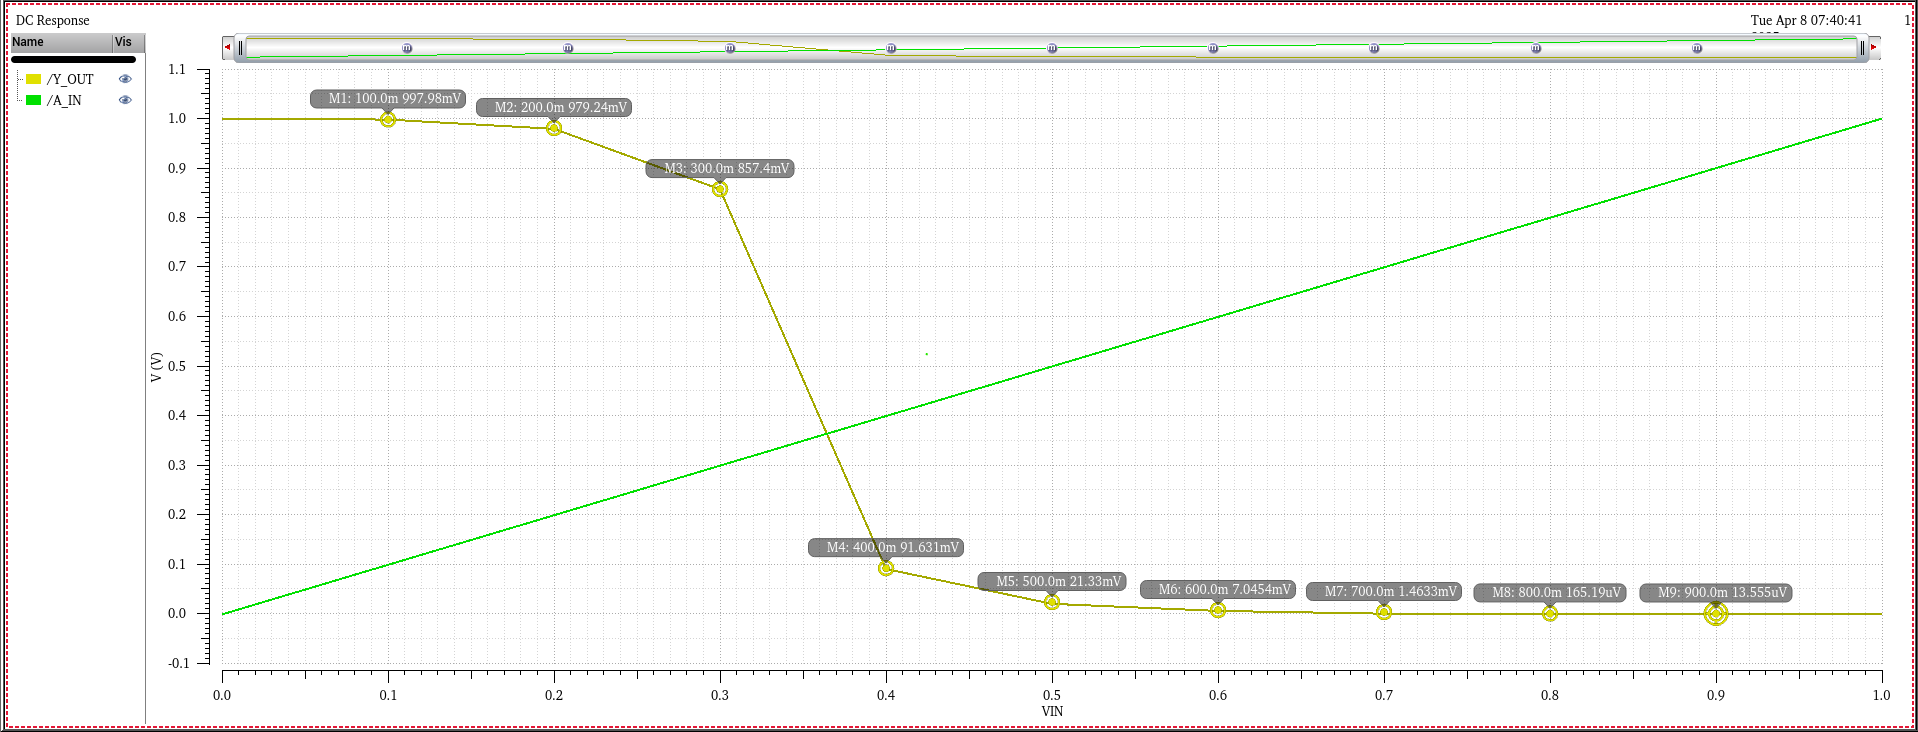
\includegraphics[width=.6\linewidth]{section/EX1/NOR/EX1_NOR2_DCanalysis_vtc.png}
	\caption{Voltage transfer curve (VTC) of NOR2.}
	\label{f_EX1_NOR2_DCanalysis_vtc}
\end{figure}

\subsubsection{Transient simulation}

\begin{figure}[H]
	\centering
	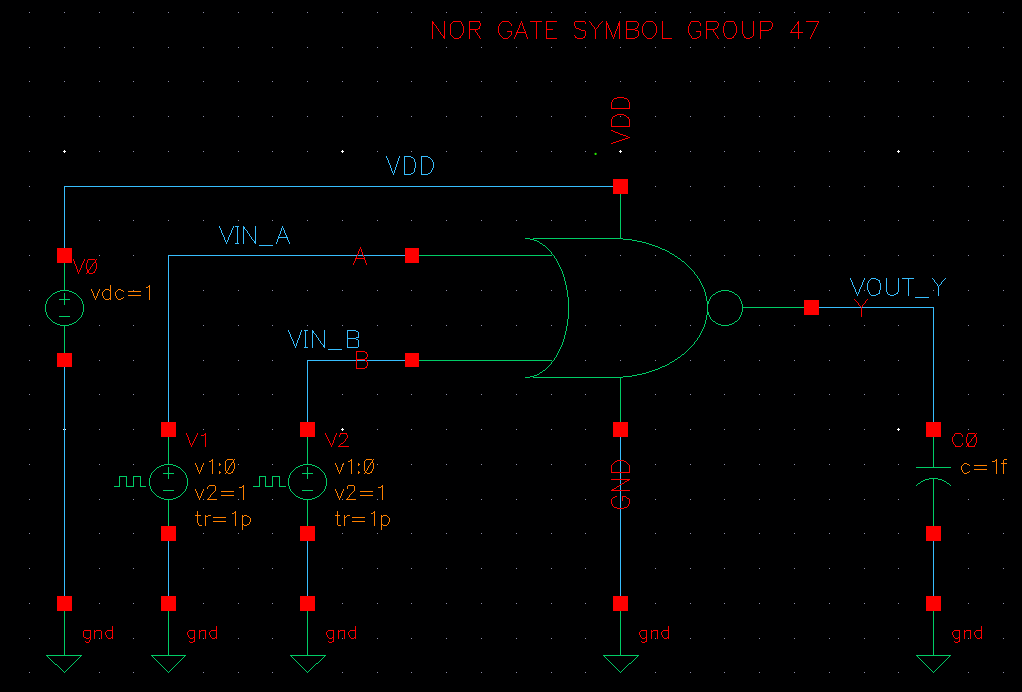
\includegraphics[width=.6\linewidth]{section/EX1/NOR/EX1_NOR2_Trans_schematic.png}
	\caption{The Circuit test NOR2.}
\end{figure}

\begin{figure}[H]
	\centering
	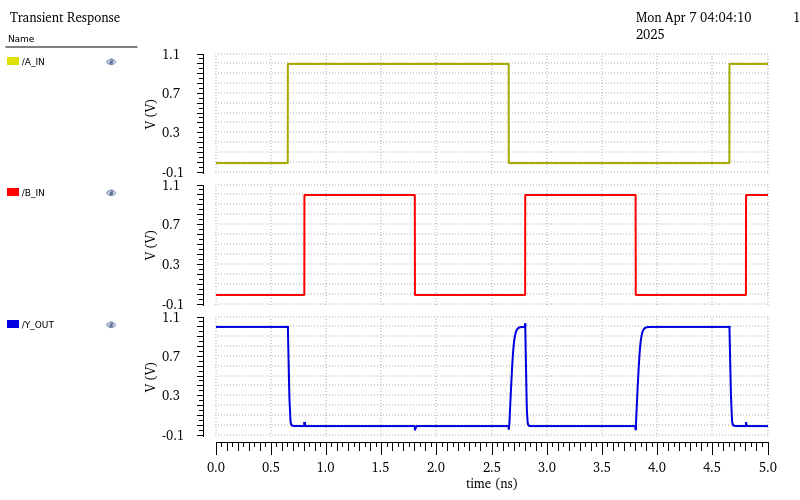
\includegraphics[width=.6\linewidth]{section/EX1/NOR/EX1_NOR2_waveform.png}
	\caption{The waveform NOR2.}
	\label{f_EX1_NOR2_waveform}
\end{figure}

\begin{table}[H]
	\centering
	\begin{tabular}{|p{.5\linewidth}|c|}
		\hline
		Parameters & Result\\
		\hline
		$t_{rise}$ - Rising time ($10\% - 90\%$) & $24.95\times10^{-12}$\\
		\hline
		$t_{fall}$  Falling time ($90\% - 10\%$) & $28.57\times10^{-12}$\\
		\hline
		$t_{pdr}$ - Rising propagation delay ($90\% - 50\%$) & $13.91\times10^{-12}$\\
		\hline
		$t_{pdf}$ - Falling propagation delay ($10\% - 50\%$) & $14.78\times10^{-12}$\\
		\hline
		$t_{p}$ - Average propagation delay ($50\% - 50\%$) & $14.35\times10^{-12}$\\
		\hline
		Power consumption & $0$\\
		\hline
	\end{tabular}
	\caption{Requirements for measuring NOR2.}
	\label{f_measuring NOR2}
\end{table}

\begin{figure}[H]
	\begin{minipage}{0.5\linewidth}
		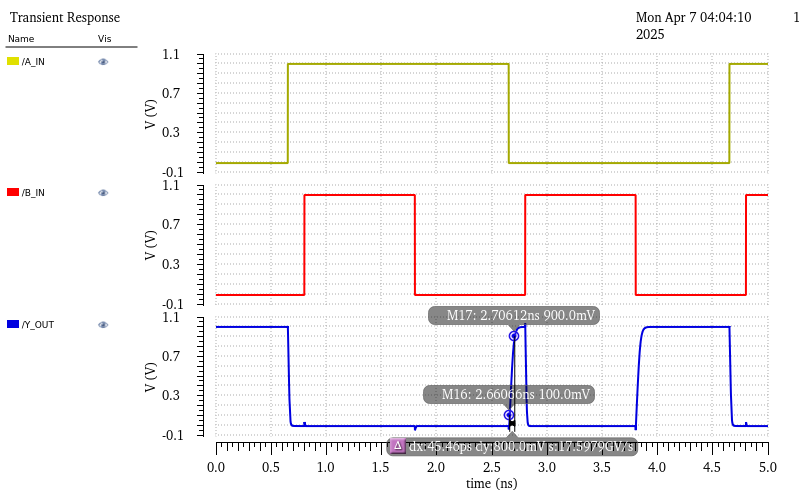
\includegraphics[width=\linewidth]{section/EX1/NOR/EX1_NOR2_Tr_Waveform.png}
	\end{minipage}
	\begin{minipage}{0.5\linewidth}
		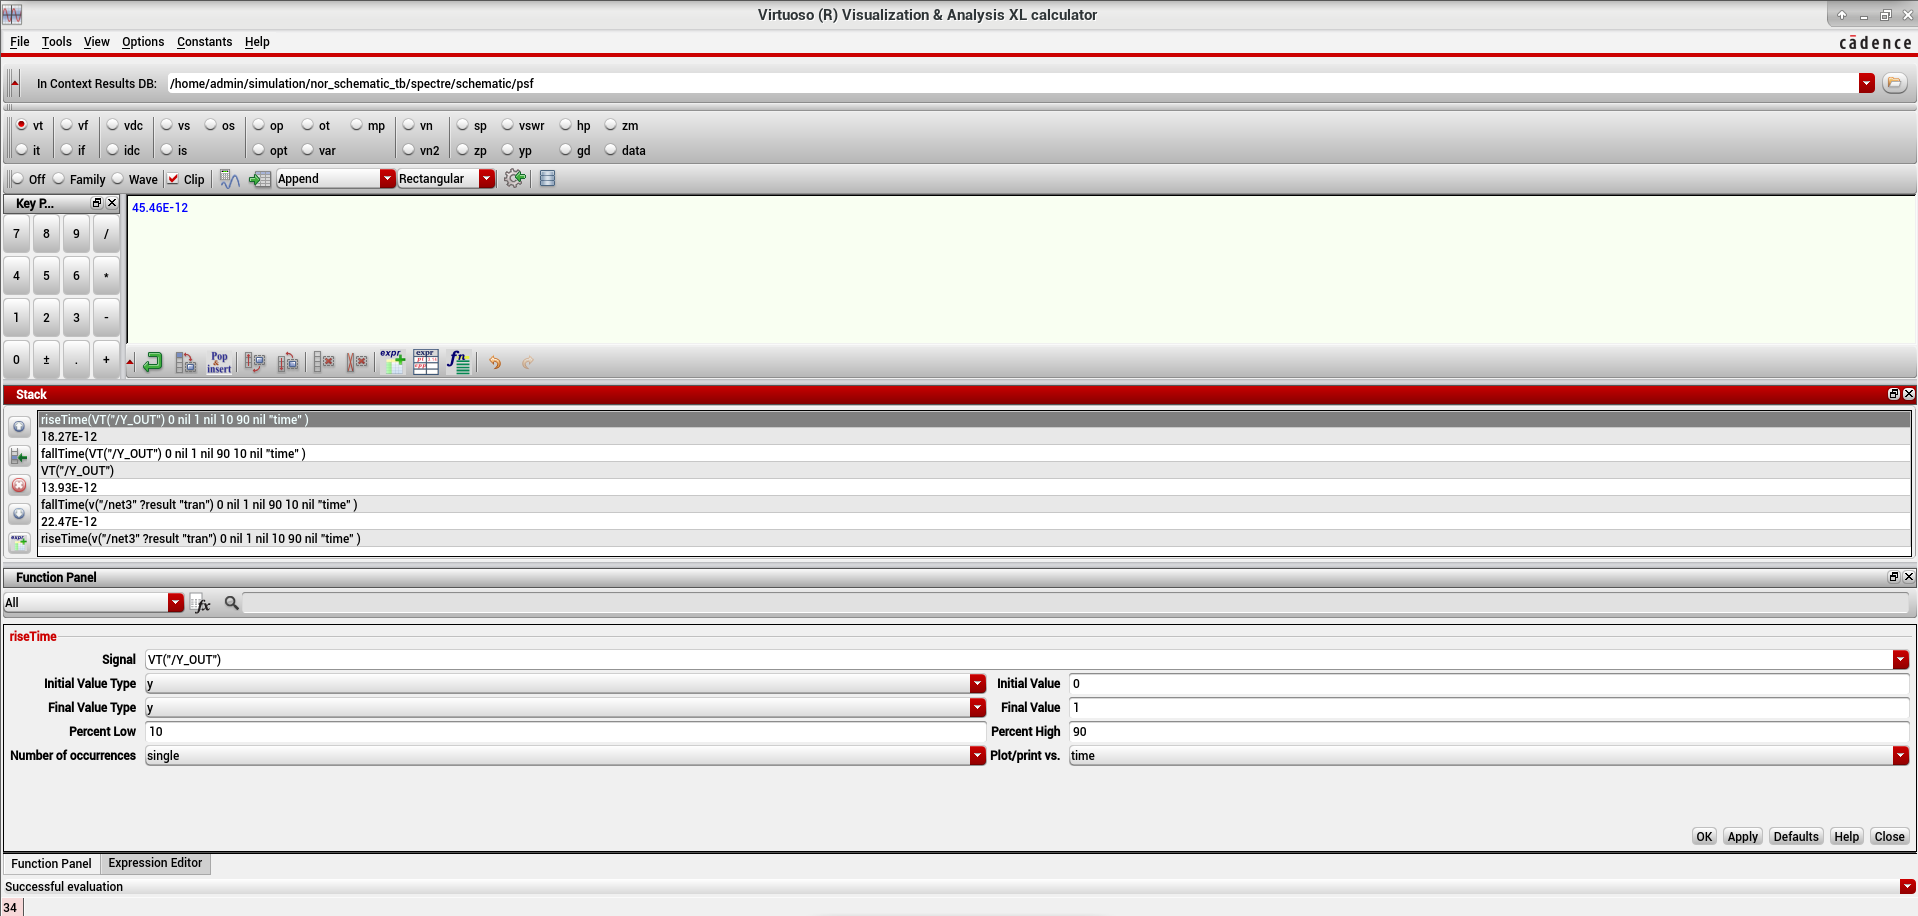
\includegraphics[width=\linewidth]{section/EX1/NOR/EX1_NOR2_Tr_Cal.png}
	\end{minipage}
	\caption{Measurement Time rising NOR2.}
\end{figure}

\begin{figure}[H]
	\begin{minipage}{0.5\linewidth}
		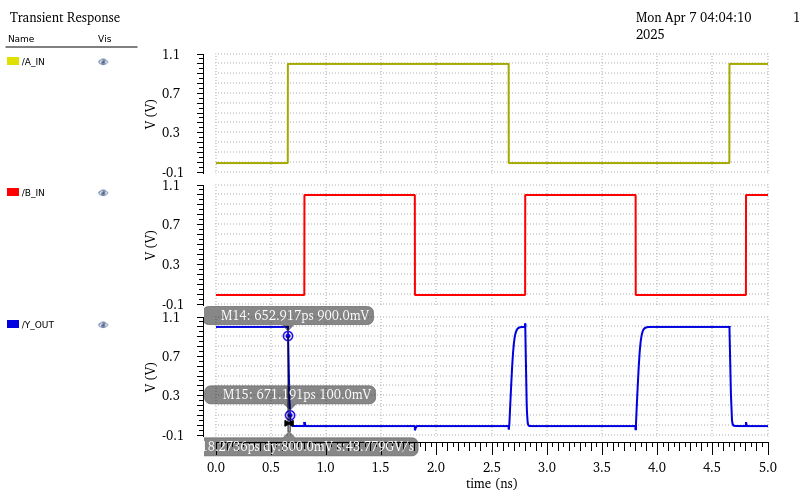
\includegraphics[width=\linewidth]{section/EX1/NOR/EX1_NOR2_Tf_Waveform.png}
	\end{minipage}
	\begin{minipage}{0.5\linewidth}
		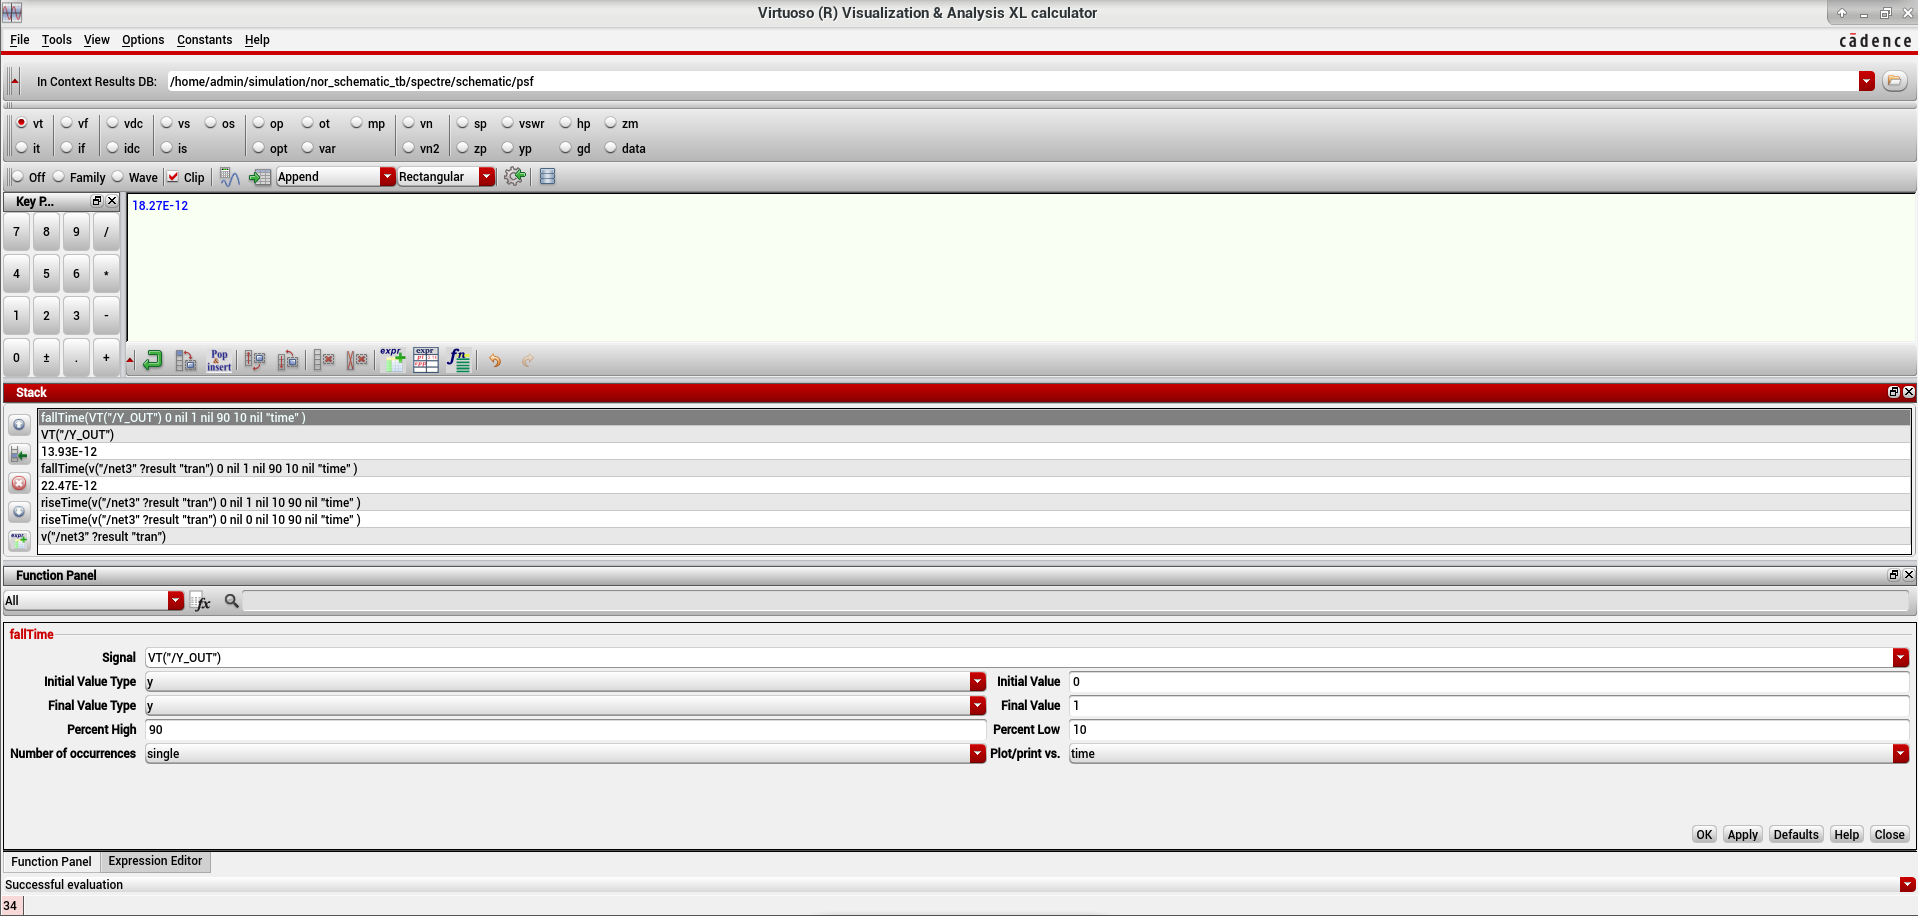
\includegraphics[width=\linewidth]{section/EX1/NOR/EX1_NOR2_Tf_Cal.png}
	\end{minipage}
	\caption{Measurement Time falling NOR2.}
\end{figure}

\begin{figure}[H]
	\begin{minipage}{0.5\linewidth}
		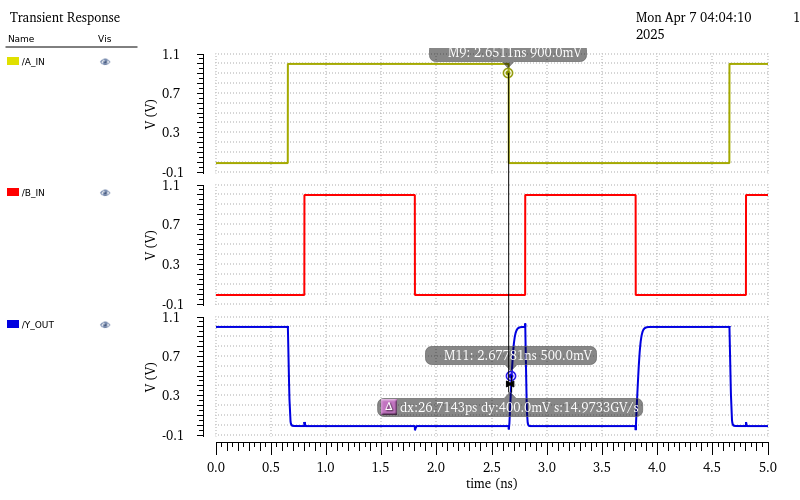
\includegraphics[width=\linewidth]{section/EX1/NOR/EX1_NOR2_Tpdr_Waveform.png}
	\end{minipage}
	\begin{minipage}{0.5\linewidth}
		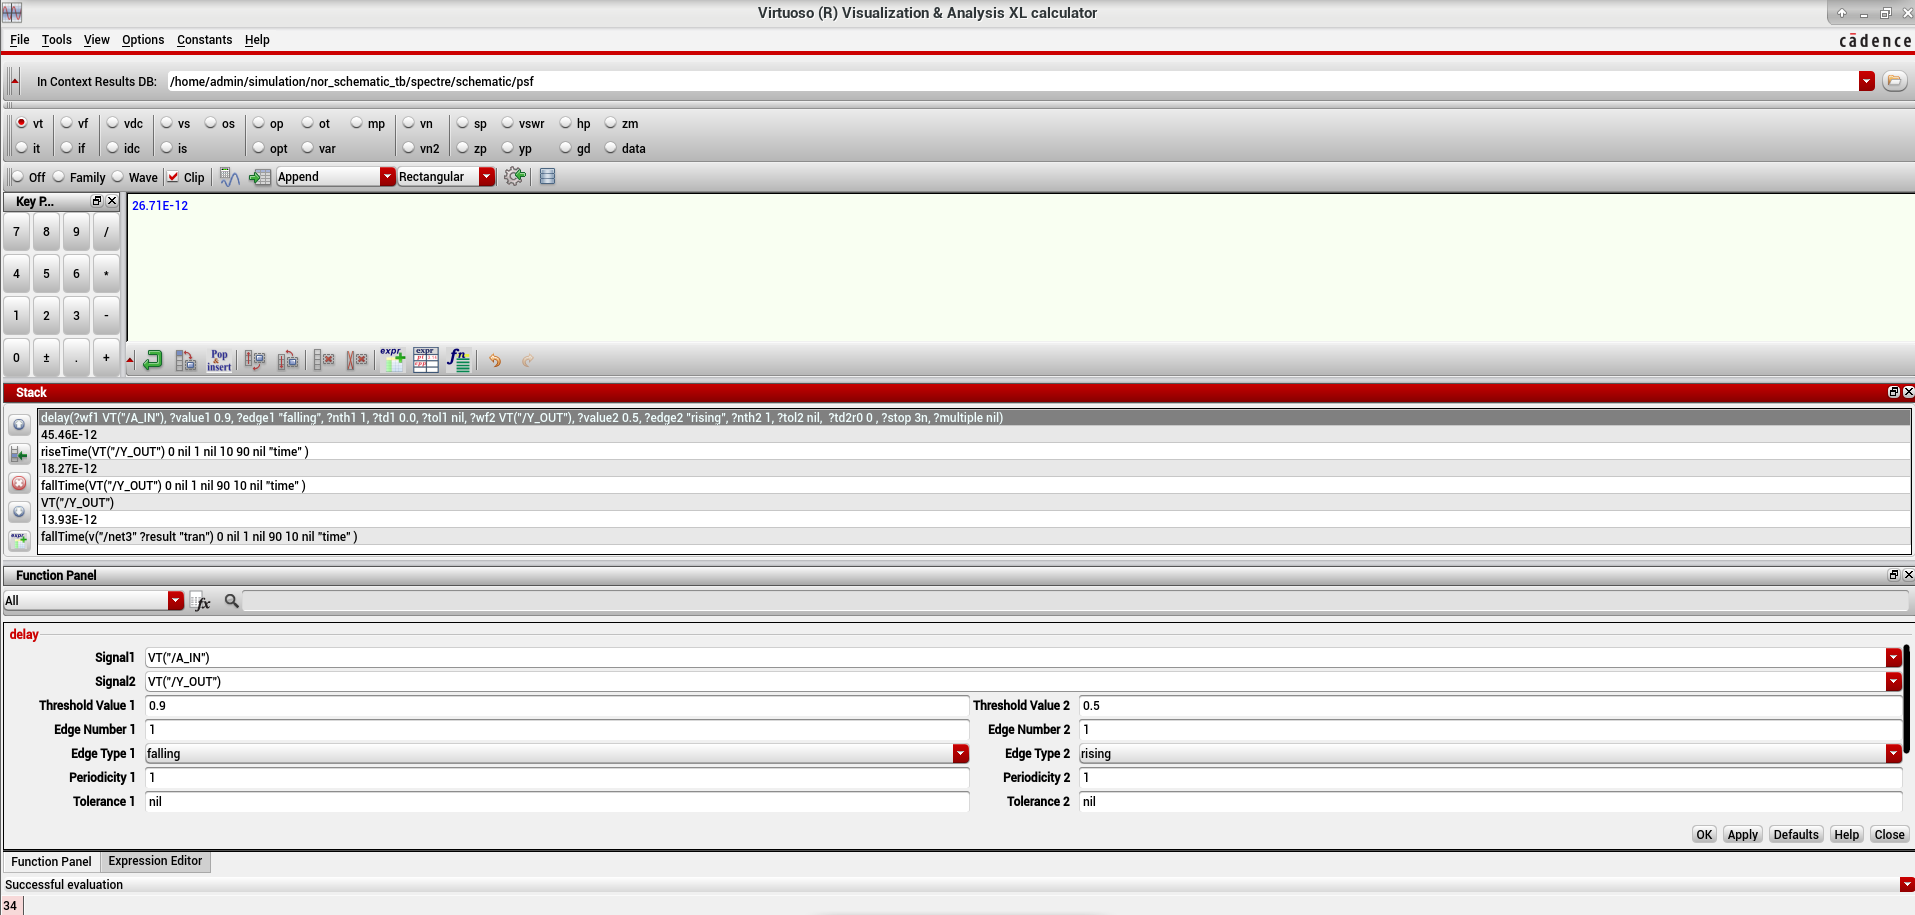
\includegraphics[width=\linewidth]{section/EX1/NOR/EX1_NOR2_Tpdr_Cal.png}
	\end{minipage}
	\caption{Measurement Time rising propagation NOR2.}
\end{figure}

\begin{figure}[H]
	\begin{minipage}{0.5\linewidth}
		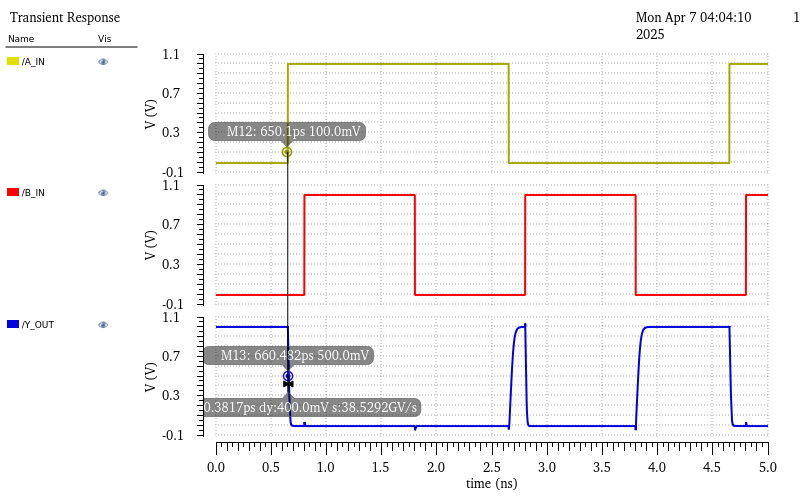
\includegraphics[width=\linewidth]{section/EX1/NOR/EX1_NOR2_Tpdf_Waveform.png}
	\end{minipage}
	\begin{minipage}{0.5\linewidth}
		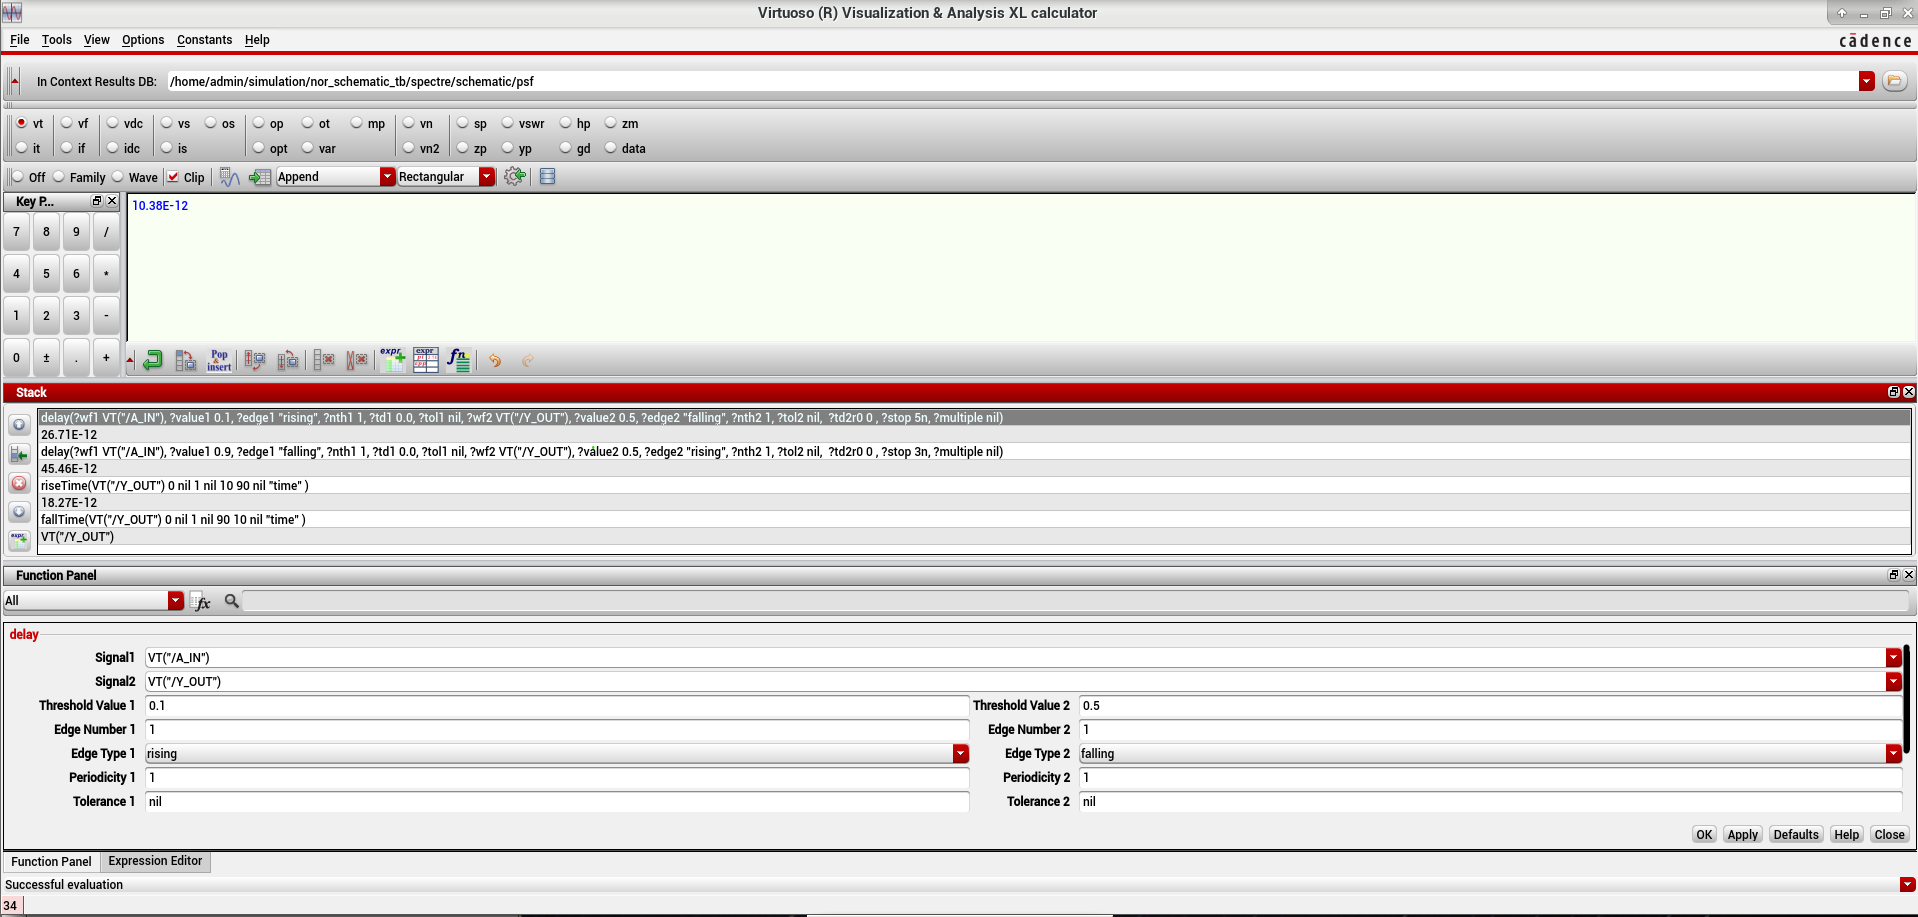
\includegraphics[width=\linewidth]{section/EX1/NOR/EX1_NOR2_Tpdf_Cal.png}
	\end{minipage}
	\caption{Measurement Time falling propagation NOR2.}
\end{figure}

\subsubsection{Layout of NOR2}

\subsection{EXOR2 gate}

\subsubsection{Schematic}

\begin{table}[H]
	\centering
	\begin{tabular}{|c|c|c|}
		\hline
		\multicolumn{2}{|c|}{INPUT} & OUTPUT \\
		\hline
		A & B  & OUT\\
		\hline
		0 & 0 & 0 \\
		\hline
		0 & 1 & 1\\
		\hline
		1 & 0 & 1\\
		\hline0
		1 & 1 & 0\\
		\hline
	\end{tabular}
	\caption{The truth table of an EXOR2.}
	\label{t_the truth table of EXOR2}
\end{table}

The schematic of a EXOR2.

\begin{figure}[H]
	\centering
	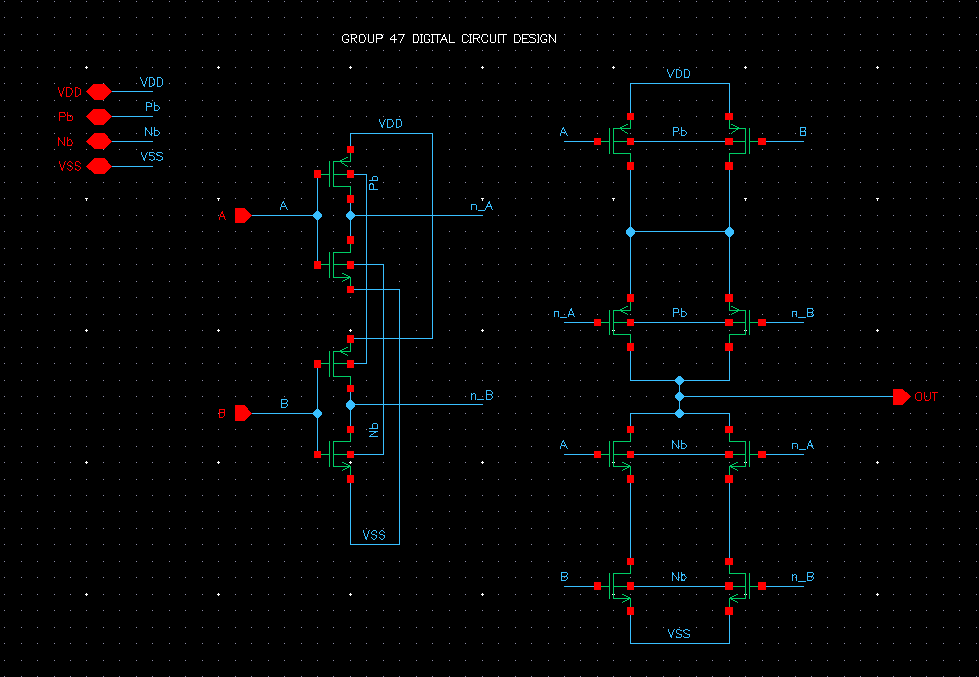
\includegraphics[width=.6\linewidth]{section/EX1/EXOR/EX1_EXOR2_schematic.png}
	\caption{The schematic of a EXOR2.}
	\label{f_EX1_EXOR2_schematic}
\end{figure} 

The symbol of a EXOR2.

\begin{figure}[H]
	\centering
	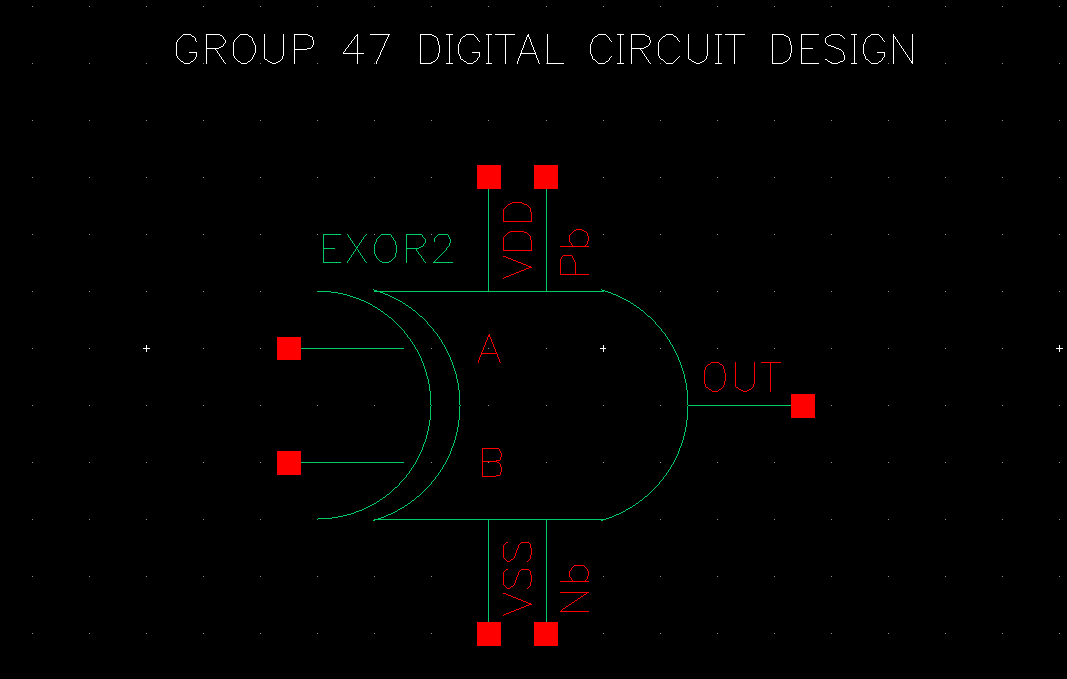
\includegraphics[width=.6\linewidth]{section/EX1/EXOR/EX1_EXOR2_symbol.png}
	\caption{The symbol of EXOR2.}
	\label{f_EX1_EXOR2_symbol}
\end{figure}

\subsubsection{DC Analysis simulation}

Use \textbf{ADE-L} to simulate the DC response of an \textit{EXOR2 gate}. Apply an input signal as a ramp voltage ranging form 0V to 1V or perform a voltage sweep from 0V to 1V. Observe the corresponding output response. The circuit parameters are configured as follows:

\begin{table}[H]
	\centering
	\begin{tabular}{|c|c|}
		\hline
		Parameters & Value \\
		\hline
		$V_{dd}$ & $1V$ \\
		\hline
		$C_{load}$ & $1fF$\\
		\hline
		$V_{in}$ & $[0, 1] V$\\
		\hline
	\end{tabular}
	\caption{Parameters in DC analysis.}
\end{table}

\begin{figure}[H]
	\centering
	\includegraphics[width=.6\linewidth]{section/EX1/EXOR/EX1_EXOR2_DCanalysis_schematic.png}
	\caption{The circuit test EXOR2.}
\end{figure}


\begin{table}[H]
	\centering
	\begin{tabular}{|c|c|c|c|c|c|c|c|c|c|}
		\hline
		$V_{in}(V)$ & $0.1$ & $0.2$ & $0.3$ & $0.4$ & $0.5$ & $0.6$ & $0.7$ & $0.8$ & $0.9$ \\
		\hline
		$V_{out}(V)$ & $100.0u$ & $111.27u$ & $214.81u$ & $2.94m$ & $880.46m$ & $142.69m$ & $33.31m$ & $15.47m$ & $618.14u$ \\
		\hline
	\end{tabular}
	\caption{The output voltage values at various values of $V_{in}$ with $0.1V$ step.}
\end{table}

\begin{figure}[H]
	\centering
	\includegraphics[width=.6\linewidth]{section/EX1/EXOR/EX1_EXOR2_DCanalysis_vtc.png}
	\caption{Voltage transfer curve (VTC) of EXOR2.}
	\label{f_EX1_EXOR2_DCanalysis_vtc}
\end{figure}

\subsubsection{Transient simulation}

\begin{figure}[H]
	\centering
	\includegraphics[width=.6\linewidth]{section/EX1/EXOR/EX1_EXOR2_Trans_schematic.png}
	\caption{The Circuit test EXOR2.}
\end{figure}

\begin{figure}[H]
	\centering
	\includegraphics[width=.6\linewidth]{section/EX1/EXOR/EX1_EXOR2_waveform.png}
	\caption{The waveform EXOR2.}
	\label{f_EX1_EXOR2_waveform}
\end{figure}

\begin{table}[H]
	\centering
	\begin{tabular}{|p{.5\linewidth}|c|}
		\hline
		Parameters & Result\\
		\hline
		$t_{rise}$ - Rising time ($10\% - 90\%$) & $58.68\times10^{-12}$\\
		\hline
		$t_{fall}$  Falling time ($90\% - 10\%$) & $39.73\times10^{-12}$\\
		\hline
		$t_{pdr}$ - Rising propagation delay ($90\% - 50\%$) & $\times10^{-12}$\\
		\hline
		$t_{pdf}$ - Falling propagation delay ($10\% - 50\%$) & $19.67\times10^{-12}$\\
		\hline
		$t_{p}$ - Average propagation delay ($50\% - 50\%$) & $\times10^{-12}$\\
		\hline
		Power consumption & $0$\\
		\hline
	\end{tabular}
	\caption{Requirements for measuring EXOR2.}
	\label{f_measuring EXOR2}
\end{table}

\begin{figure}[H]
	\begin{minipage}{0.5\linewidth}
		\includegraphics[width=\linewidth]{section/EX1/EXOR/EX1_EXOR2_Tr_Waveform.png}
	\end{minipage}
	\begin{minipage}{0.5\linewidth}
		\includegraphics[width=\linewidth]{section/EX1/EXOR/EX1_EXOR2_Tr_Cal.png}
	\end{minipage}
	\caption{Measurement Time rising EXOR2.}
\end{figure}

\begin{figure}[H]
	\begin{minipage}{0.5\linewidth}
		\includegraphics[width=\linewidth]{section/EX1/EXOR/EX1_EXOR2_Tf_Waveform.png}
	\end{minipage}
	\begin{minipage}{0.5\linewidth}
		\includegraphics[width=\linewidth]{section/EX1/EXOR/EX1_EXOR2_Tf_Cal.png}
	\end{minipage}
	\caption{Measurement Time falling EXOR2.}
\end{figure}

\begin{figure}[H]
	\begin{minipage}{0.5\linewidth}
		\includegraphics[width=\linewidth]{section/EX1/EXOR/EX1_EXOR2_Tpdr_Waveform.png}
	\end{minipage}
	\begin{minipage}{0.5\linewidth}
		\includegraphics[width=\linewidth]{section/EX1/EXOR/EX1_EXOR2_Tpdr_Cal.png}
	\end{minipage}
	\caption{Measurement Time rising propagation EXOR2.}
\end{figure}

\begin{figure}[H]
	\begin{minipage}{0.5\linewidth}
		\includegraphics[width=\linewidth]{section/EX1/EXOR/EX1_EXOR2_Tpdf_Waveform.png}
	\end{minipage}
	\begin{minipage}{0.5\linewidth}
		\includegraphics[width=\linewidth]{section/EX1/EXOR/EX1_EXOR2_Tpdf_Cal.png}
	\end{minipage}
	\caption{Measurement Time falling propagation EXOR2.}
\end{figure}

\subsubsection{Layout of EXOR2}

\begin{figure}[H]
	\centering
	\includegraphics[width=.7\linewidth]{section/EX1/EXOR/EX1_EXOR2_layout.png}
	\caption{Layout for EXOR2.}
	\label{f_EX1_EXOR_layout}
\end{figure}

\begin{figure}[H]
	\centering
	\includegraphics[width=.7\linewidth]{section/EX1/EXOR/EX1_EXOR2_LVS_check.png}
	\caption{Check LVS for EXOR2.}
	\label{f_EX1_EXOR_LVS_check}
\end{figure}`
\end{document}